% GENERATED by paper/tex/build_tex.mjs — do not edit by hand.
%% The supplement carries its own preamble. It needs the same three settings
%% the manuscript needs, for the same reasons: authoryear so citep matches
%% elsarticle-harv rather than printing bracketed numbers against an
%% author-year list; emergencystretch so a long 	exttt path is set loose
%% rather than protruding; single-spaced float captions so a long caption
%% does not push the folio into its own text.
\documentclass[preprint,authoryear,12pt,a4paper]{elsarticle}
\usepackage[utf8]{inputenc}
\usepackage[T1]{fontenc}
\usepackage{lmodern}
\usepackage{textcomp}
\usepackage{tabularx}
\graphicspath{{../}{../figures/}{./}{./figures/}}
\usepackage{graphicx}\usepackage{amsmath}\usepackage{booktabs}\usepackage{array}
\usepackage{setspace}
\usepackage{etoolbox}
\AtBeginEnvironment{figure}{\singlespacing}
\AtBeginEnvironment{table}{\singlespacing}
\emergencystretch=3em
\renewcommand{\thetable}{S\arabic{table}}
\renewcommand{\thefigure}{S\arabic{figure}}
% Section numbers S1, S1.1 ... are part of the headings themselves.
\setcounter{secnumdepth}{0}
\usepackage{xr}
\externaldocument[M-]{manuscript}
\begin{document}

\section{Supplementary Material}

Supplementary material for \emph{Evaluation geometry and the limits of cross-region transfer in pre-fire thermal wildfire prediction}.

Section S1 reports the sensitivity analyses and the elaborations of the Results; Section S2 the supporting tables; Section S3 the protocol detail and the thirteen limitations; Section S4 the record of the transferability diagnostics; Section S5 the target-label recovery curve. Tables are numbered in order of appearance (Table~\ref{tab:S1}--S22), independently of the sections.

\textbf{Status.} Nothing in this document is evidence the paper's claims depend on that is unavailable elsewhere; every number here also appears in a frozen artefact named in the text. It is released so that a reader who wants the fuller argument, the per-scar and per-direction detail, or the exact protocol can have it without the paper carrying twenty thousand words of it.

\setcounter{tocdepth}{2}
\tableofcontents
\clearpage

\section{S1 Sensitivity analyses}

Each arm below varies one design choice and leaves everything else fixed. None changes a conclusion in the main text. They are reported so that a reader can see which choices were tested, and what each was worth. Arm (f) is the exception in one respect: it is not a robustness check but a test of a claim the introduction makes, and the claim is not upheld.

Each arm is labelled by its letter below, and is cited elsewhere in the paper as Section S1.1 through S1.8.

\subsection{S1.1 Evia AOI and prevalence}

The raw transfer arms were repeated with the legacy, high-prevalence Evia box. Every qualitative conclusion is unchanged. Thermal raw transfer AUCs move by up to 0.07, the largest being Evia to Bejís at 0.378 to 0.448, and no direction changes side of the chance line.

\subsection{S1.2 CORAL regularisation, including the canonical $\lambda$ = 1}

Over nine $\lambda$ values from 0 to 10$^{-1}$ on four directions, CORAL transfer AUC moves by at most 0.014 within any direction and 0.008 within the thermal family. The canonical $\lambda$ = 1 of the cited method lies outside that sweep and was computed separately on the same four directions. It changes the thermal mean from 0.519 to 0.522, a shift of +0.003 with a per-direction range of $-$0.005 to +0.016, and none of those four directions crosses the chance line. The $\lambda$ = 1 values are 0.510, 0.444, 0.559 and 0.575 against 0.508, 0.445, 0.564 and 0.559 at $\lambda$ = 0.1.

\textbf{Those four directions are Bejís--Muğla and Manavgat--Muğla, and they exclude the pair that moves.} An earlier version of this section generalised from them to the whole matrix, which was an error: the Manavgat--Bejís pair is not in the sweep and it is the pair whose CORAL result is $\lambda$-dependent. A separate frozen artefact, \texttt{experiments/\allowbreak{}cross\_\allowbreak{}region/\allowbreak{}step10/\allowbreak{}coral\_\allowbreak{}lambda\_\allowbreak{}sensitivity.\allowbreak{}csv}, carries it. Bejís to Manavgat gives 0.5571 [0.5292, 0.5857] at $\lambda$ = 10$^{-5}$, 0.5644 at $\lambda$ = 10$^{-3}$ and 0.5473 at $\lambda$ = 0.1, all with intervals entirely above 0.5, but \textbf{0.4850 [0.4496, 0.5197] at $\lambda$ = 1}, which crosses the chance line and loses its interval support. Manavgat to Bejís falls likewise, from 0.5108 to 0.4776 [0.4501, 0.5013].

The correct statement is therefore narrower. CORAL-dependent conclusions are insensitive to $\lambda$ over three orders of magnitude below 0.1; at the cited method's canonical $\lambda$ = 1 the one direction whose adapted interval sits entirely above chance loses that status. $\lambda$ = 10$^{-5}$ is the minimally regularised choice and matches the reference implementation, but the dependence is real and is reported rather than absorbed.

\subsection{S1.3 Blocking scale}

Recomputing the transfer quantities at 10-cell ($\approx$ 5 km) blocking from the re-frozen per-cell predictions (corrected Manavgat label) widens the intervals and moves the paired-delta verdict counts, from twelve positive, seven negative and one uncertain at 1 km to six, five and nine at 5 km. Coarser blocking therefore removes support from eight verdicts and adds none. Across five seeds the 5 km counts run 5 to 6 positive, 4 to 5 negative and 9 to 11 uncertain, so they are not exact (\texttt{paper/\allowbreak{}labelfix\_\allowbreak{}rerun/\allowbreak{}round5/\allowbreak{}out\_\allowbreak{}official/\allowbreak{}transfer\_\allowbreak{}ci\_\allowbreak{}blocksize.\allowbreak{}csv}, \texttt{paper/\allowbreak{}labelfix\_\allowbreak{}rerun/\allowbreak{}round6/\allowbreak{}seed\_\allowbreak{}stability.\allowbreak{}json}).

The point estimates are unchanged. That is an identity rather than a result, and it should not be offered as robustness. The blocking scale is the bootstrap \emph{resampling unit}, and each point estimate is computed once over all target cells, so no choice of block size could have moved one. The comparison does establish two things. Every verdict that changes, changes towards ``no verdict''. And no direction crosses the chance line under the widened intervals. The counts are the fragile part of this paper. The sign pattern is not thereby shown to be robust. It is simply not tested by this variation.

\textbf{Table~\ref{M-tab:1} note (resampling units), moved from Section~\ref{M-sec:4.2}.} The bootstrap resamples spatial blocks. An interval's reliability is therefore bounded by the number of blocks carrying at least one burned cell. Those counts fall from 192 to 843 at 2 cells to \textbf{6 to 33} at 20 cells. An interval built on six such blocks has no meaningful coverage, so \textbf{the 20-cell row should be read as indicative rather than as an interval}. The 10-cell row is the coarsest blocking this design supports properly. Every region there has 16 to 70 positive-carrying blocks, and the increment holds at that scale in all five regions (above).

\subsection{S1.4 Predictor-window closure}

The predictor window was closed 7 and 14 days earlier in all five regions. The thermal contribution stays positive and bootstrap-supported everywhere. The direction of the change is region-specific. It strengthens in Bejís, from 0.058 to 0.079 at 14 days, and in Muğla, from 0.115 to 0.128. It is flat in Montiferru. It weakens monotonically in Evia, from 0.156 to 0.149 to 0.135. What holds in every region is survival, not improvement. That is the claim carried in Section~\ref{M-sec:5.2}.

\subsection{S1.5 Quality screening of the coarse thermal input}

Two of the five regions' MODIS inputs are quality-screened and three are not. The split follows export date rather than design, and it induces an elevation-correlated change at the input, at r = +0.615 in Manavgat. On 14 August 2026, under the frozen label, Manavgat's downstream chain was rebuilt from a quality-screened input. That changes the downscaled surface on 22,304 of 24,150 cells, by up to 10.9 \textdegree{}C. No signed univariate association moved by more than +0.0003. Elevation was identical in both arms, at 0.374, the population was unchanged, and the within-region increment moved from [+0.055, +0.079] to [+0.054, +0.077]. The description of that run as rebuilding both arms with the same code was almost certainly inaccurate: the current step7 refuses the unscreened raster, so the unscreened arm ran the step7 of export time and the two arms differed in code version as well as in screening (Section~\ref{M-sec:3.4}). Its Muğla arm was not re-examined. On the corrected label the comparison is reported in Section~\ref{M-sec:3.4}. The reason is structural. Elevation is a DEM variable the screening cannot touch, and fusion falls back on the MODIS-derived surface across only 2.14 percentage points of coverage. Details are in \texttt{paper/\allowbreak{}modis\_\allowbreak{}qc\_\allowbreak{}downstream\_\allowbreak{}propagation.\allowbreak{}md}.

\textbf{Quality screening, and a correction (moved from Methods 3.4).} The MODIS surface temperature behind the downscaled and fused channels entered Manavgat's frozen export unscreened. Section S1.5 compares that arm with a screened one on the corrected label. The current pipeline's step7 refuses the unscreened raster, because it carries no nodata tag and 8.1 \% exact zeros. The unscreened arm therefore runs the step7 of export time and the screened arm the current one, so the two differ in code version as well as in screening. The earlier version of this comparison, run on 14 August 2026, described both arms as rebuilt with the same code. That was almost certainly inaccurate: its unscreened arm would have met the same refusal, and its signed AUCs equal the frozen ones. Its Muğla arm was not re-examined. The result does not change. Elevation stays at 0.232, no other signed AUC moves by more than 0.005 (downscaled LST, $-$0.0044), and the within-region increment moves from +0.067 to +0.068 (Section S3.5(xii)).

\subsection{S1.6 Normalised against absolute dryness channels}

Section~\ref{M-sec:1.2} argues that an internally normalised index should be less exposed to absolute-temperature offsets between regions than raw land surface temperature. The thermal block contains both kinds, so the argument can be tested directly as a feature-set contrast.

One thing should be said before the result, because it makes the outcome less surprising than it might otherwise appear. The normalised channels are the two that hold their direction in the same-geography two-event comparison of Section S1.13, where the absolute channels move. That is a statement about one region across two fires. \textbf{Across regions it does not hold}: \texttt{lst\_\allowbreak{}anomaly\_\allowbreak{}mean} is itself one of the seven predictors whose reversal is bootstrap-supported on the frames as drawn (Table~\ref{tab:S10}), reversing between Bejís and Evia (Section~\ref{M-sec:4.4} withdraws that support under an equalised frame), which is why Section S1.14 drops it alongside elevation. Being internally normalised protects a channel against the offset between two seasons in one place. It does not, on this evidence, protect it against a change of place.

Three feature sets were run over all twenty directions and all five within-region folds, with the classifier, population, folds and bootstrap held fixed. The harness aborts unless its reference configuration lands on the re-frozen exports (corrected Manavgat label). It did exactly: the maximum absolute difference between the reference arm and the step9b transfer AUCs is 0.000000 across all twenty directions (\texttt{paper/\allowbreak{}labelfix\_\allowbreak{}rerun/\allowbreak{}round3/\allowbreak{}no\_\allowbreak{}coord\_\allowbreak{}channels.\allowbreak{}json}).

\begin{center}
  \small
  \begin{tabularx}{\linewidth}{>{\raggedright\arraybackslash}Xrr>{\raggedleft\arraybackslash}X}
    \hline
    Feature set & Mean transfer AUC & Directions > 0.5 & Mean within-region AUC \\
    \hline
    baseline only & 0.5194 & 13 & 0.7973 \\
    baseline + normalised anomalies & 0.5245 & 14 & 0.8621 \\
    baseline + absolute surface state & 0.5308 & 13 & 0.8641 \\
    all ten features (reference) & 0.5267 & 13 & 0.8959 \\
    \hline
  \end{tabularx}
\end{center}

\textbf{The advantage is not found.} Per direction, the normalised set minus the absolute set has a mean of $-$0.0063. It is positive in 11 of 20 directions and runs from $-$0.099 to +0.087, so the spread is an order of magnitude larger than the difference. The normalised channels transfer very slightly worse at the mean, and nothing here supports a design rule favouring anomaly-referenced dryness for portability.

Within region the two sub-blocks are indistinguishable, at 0.8621 and 0.8641, and each recovers most of the gap between the baseline's 0.7973 and the full model's 0.8959. What separates them in sign stability does not become transferable skill.

This arm strengthens the negative finding rather than softening it. Four differently constituted feature sets were tried. None clears a mean of 0.531 across regions, and all differ sharply within them. The baseline arm also gives an independent confirmation of the control reported in Section~\ref{M-sec:4.5}: its mean transfer of 0.5194 was recomputed here from the modelling datasets and matches the 0.519 of the re-frozen per-direction export. Details are in \texttt{paper/\allowbreak{}anomaly\_\allowbreak{}only\_\allowbreak{}transfer.\allowbreak{}md}.

The comparison is between two sub-blocks of one thermal set on one cohort. It does not test normalised dryness indices in general, and it does not test a normalisation fitted against a pooled multi-region reference rather than each region's own baseline years.

\subsection{S1.7 The coordinate-informed channels}

\texttt{downscaled\_\allowbreak{}lst\_\allowbreak{}mean} and \texttt{fused\_\allowbreak{}lst\_\allowbreak{}mean} come from a per-region downscaling model whose own inputs include coordinates, which Section~\ref{M-sec:3.13} names as the one route by which a coordinate-derived surface re-enters a feature set that excludes coordinates. A coordinate-smoothed surface is by construction locally informative and non-portable, so if the within-region increment depended on it, that increment would be this paper's own result in miniature rather than a finding about thermal dryness. The arm was therefore run here rather than deferred.

Both channels were dropped and everything refitted, over all twenty directions and all five within-region folds. The reference configuration reproduces the frozen exports exactly, at 0.000000 against both the transfer and the within-region references.

\begin{center}
  \small
  \begin{tabularx}{\linewidth}{lr>{\raggedleft\arraybackslash}Xr}
    \hline
    Region & Increment, full set & Increment without the two channels & Retained \\
    \hline
    Manavgat 2021 & +0.067 & +0.063 & 94 \% \\
    Bejís 2022 & +0.056 & +0.046 & 82 \% \\
    Muğla 2021 & +0.116 & +0.097 & 84 \% \\
    North Evia 2021 & +0.153 & +0.145 & 94 \% \\
    Montiferru 2021 & +0.101 & +0.105 & 103 \% \\
    \textbf{Mean} & \textbf{+0.099} & \textbf{+0.091} & \textbf{92 \%} \\
    \hline
  \end{tabularx}
\end{center}

\textbf{The increment does not depend on them.} It stays positive in every region and retains 82 \% to 103 \% of its size, rising slightly in one region. Mean transfer is likewise unchanged, at 0.545 without the two channels against 0.541 with them and 0.537 for the baseline alone. The local skill this paper reports is therefore not an artefact of a coordinate-smoothed surface.

This arm was computed independently here and reproduces the companion paper's figure for the same quantity, 82 \% to 103 \%, from a separately written harness.

\subsection{S1.8 Model capacity}

Every number in this paper comes from one random forest with unlimited depth and \texttt{min\_\allowbreak{}samples\_\allowbreak{}leaf = 3}. That is the configuration most able to encode local structure and least able to extrapolate, so a reader may reasonably ask whether the transfer failure is a property of the predictors or of the estimator. Holding the model fixed is right for the internal comparisons and does not license the external claim, so three further estimators were run over the same twenty directions and the same five within-region folds.

\begin{center}
  \footnotesize
  \resizebox{\ifdim\width>\linewidth\linewidth\else\width\fi}{!}{%
  \begin{tabular}{lrrrrr}
    \hline
    Estimator & Within-region AUC & Within increment & Transfer AUC & Transfer increment & Above chance \\
    \hline
    Random forest, depth unlimited, leaf 3 & 0.888 & +0.099 & 0.541 & +0.004 & 14 of 20 \\
    Random forest, depth 6, leaf 50 & 0.829 & +0.055 & \textbf{0.556} & $-$0.007 & 14 of 20 \\
    Random forest, leaf 200 & 0.805 & +0.047 & \textbf{0.550} & $-$0.021 & 14 of 20 \\
    Penalised logistic regression & 0.741 & +0.045 & \textbf{0.510} & $-$0.024 & 14 of 20 \\
    \hline
  \end{tabular}}
\end{center}

\textbf{Regularisation does not rescue transfer.} All four estimators land between 0.510 and 0.556, all four put exactly fourteen of twenty directions above chance, and the linear model, the one built to extrapolate, transfers worst. Within-region skill falls as capacity is reduced, from 0.888 to 0.741, which is what regularisation is expected to cost; transfer does not rise to meet it. The thermal block's contribution to transfer is +0.004 under the canonical forest and \textbf{negative} under all three regularised alternatives, so the block does not become portable when the model is made simpler.

The transfer failure is therefore a property of the predictors on this cohort, not of an unregularised forest. Detail in \texttt{paper/\allowbreak{}model\_\allowbreak{}capacity.\allowbreak{}json}.

\subsection{S1.9 The four evaluations of Section~\ref{M-sec:4.3}, in full}

Section~\ref{M-sec:4.3} reports four evaluations of the same models as a ladder. The per-split and per-scar detail is here, so that the ladder can be checked without leaving the manuscript.

\begin{table}[htbp]
  \centering
  \footnotesize
  \caption{The four evaluations, scored on identical cells. Primary natural-vegetation population. Rows B, C and D are scored on the held-out scar area; row A is the whole region and is shown to make the mismatch visible. Means and Student \emph{t} intervals are over the seven held-out scars.}
  \label{tab:S1}
  \begin{tabularx}{\linewidth}{>{\raggedright\arraybackslash}X>{\raggedright\arraybackslash}Xlrl}
    \hline
    Evaluation & Model trained on & Scored on & Mean AUC & 95 \% CI \\
    \hline
    A. Blocked cross-validation, 5 km & the region, scar included & the whole region & 0.773 & [0.729, 0.818] \\
    B. Same blocked model, restricted & the region, \textbf{scar included} & the scar area & 0.640 & [0.544, 0.736] \\
    C. Leave-one-scar-out & the region, \textbf{scar withheld} & the scar area & 0.546 & [0.488, 0.604] \\
    D. Foreign region & another region, 306 to 2,802 km & the scar area & 0.553 & [0.495, 0.611] \\
    \hline
  \end{tabularx}
\end{table}

\subsubsection{S1.9.1 Where the skill is lost, on a matched comparison}

\textbf{Where the skill is lost, on a matched comparison.} Four evaluations are reported. The last three are scored on \textbf{identical cells}, so they differ only in what the model was trained on. The first shows why an unmatched comparison misleads. The held-out unit is a burned connected component of at least 50 cells, with all cells within 2 km of it. What makes that harder than a whole region is the composition of its negatives, not its burned fraction, and that is measured rather than argued. The same predictions were scored on a random sample of region cells drawn at the scar area's own burned fraction. That gives \textbf{0.793 against the region-wide 0.791}, so matching prevalence changes nothing, at $-$0.002 [$-$0.005, +0.001]. Scoring them on the scar area gives 0.644, a fall of \textbf{+0.149 [+0.087, +0.211]}. That swaps both pools at once, so each was swapped singly. Replacing only the negatives costs \textbf{0.139 [0.098, 0.181]}, the whole of it. Replacing only the positives costs \textbf{$-$0.002 [$-$0.055, +0.051]}, null on average, though the per-scar effect runs from $-$0.12 to +0.14. \textbf{The effect is the negative pool.} Every negative in a scar collar is fire-adjacent and shares the terrain, land cover and synoptic conditions of the positives, whereas a region's negatives include its easy far field. ROC-AUC is in any case invariant to class balance at fixed class-conditional distributions (\texttt{pool\_\allowbreak{}decomposition.\allowbreak{}json}).

\subsubsection{S1.9.2 The seven scars and the resampling unit}

All four rows are means over the \textbf{same seven scars}. Bejís and Manavgat have no row C, because in each the burned area is a single component, so withholding it leaves nothing to train on. Under the corrected label the 2,151 added Manavgat burns merge into its one existing scar (2,934 of 2,935 cells). That is why the controls above are computed on nine scars and report 0.791 and 0.644 against Table~\ref{tab:S1}'s 0.773 and 0.640. The intervals are Student \emph{t} over the scars. That is this arm's resampling unit, rather than the spatial-block bootstrap used elsewhere. Four scars are in Muğla, two in Montiferru and one in Evia. \textbf{Row A is a region-level quantity repeated identically across a region's scars, so its interval is pseudo-replicated and should not be read as coverage.} That repetition propagates into A $-$ B and A $-$ C. Clustering by region, over three regions, gives \textbf{+0.137 [+0.048, +0.226]} and \textbf{+0.266 [$-$0.022, +0.553]}. The first still excludes zero. The second no longer does, and is 3.6 times wider. \textbf{The scar-level intervals on these two differences therefore overstate precision, and on the region unit only the frame cost is established} (Section S1.9).

\subsubsection{S1.9.3 Controls, full specification}

Three controls reuse A's predictions, each averaged over 20 draws without replacement. The \textbf{prevalence-matched} control draws $|H_K^{+}|$ cells from $P_R$ and $|H_K^{-}|$ from $V_R \setminus P_R$. The \textbf{negative-pool} control keeps the drawn burned cells but uses the scar's own negatives $H_K^{-}$, and the positive-pool control does the converse. A \textbf{within-region half-split} (modelled cells cut at the median of a grid axis, both axes and directions, a split discarded when either half is single-class) completes the set, under the transfer protocol of Section~\ref{M-sec:3.8} unchanged. The per-split and per-scar positive counts are unequal and bear on the interpretation (Table~\ref{tab:S2} below).

\begin{table}[htbp]
  \centering
  \scriptsize
  \caption{Within-region half-split, every split. Source and target positive counts are given because they are unequal, which is the principal limit on this arm: a straight cut does not produce two exchangeable halves. Two splits are unusable because one half of Manavgat contains no burned cells. Corrected Manavgat label; source \texttt{paper/\allowbreak{}labelfix\_\allowbreak{}rerun/\allowbreak{}code/\allowbreak{}positive\_\allowbreak{}control.\allowbreak{}json}. Checked row by row by \texttt{paper/\allowbreak{}code/\allowbreak{}appendix\_\allowbreak{}tables.\allowbreak{}py}.}
  \label{tab:S2}
  \resizebox{\ifdim\width>\linewidth\linewidth\else\width\fi}{!}{%
  \begin{tabular}{lllrrrr}
    \hline
    Region & Axis & Direction & Source positives & Target positives & Thermal AUC & Baseline AUC \\
    \hline
    manavgat 2021 & east-west & low to high & 1,795 & 1,140 & 0.761 & 0.793 \\
    manavgat 2021 & east-west & high to low & 1,140 & 1,795 & 0.712 & 0.638 \\
    manavgat 2021 & north-south & low to high & 0 & 2,935 & --- & --- \\
    manavgat 2021 & north-south & high to low & 2,935 & 0 & --- & --- \\
    bejis 2022 & east-west & low to high & 640 & 460 & 0.750 & 0.784 \\
    bejis 2022 & east-west & high to low & 460 & 640 & 0.578 & 0.560 \\
    bejis 2022 & north-south & low to high & 357 & 743 & 0.713 & 0.662 \\
    bejis 2022 & north-south & high to low & 743 & 357 & 0.603 & 0.613 \\
    mugla 2021 & east-west & low to high & 1,449 & 1,462 & 0.448 & 0.378 \\
    mugla 2021 & east-west & high to low & 1,462 & 1,449 & 0.636 & 0.628 \\
    mugla 2021 & north-south & low to high & 774 & 2,137 & 0.533 & 0.503 \\
    mugla 2021 & north-south & high to low & 2,137 & 774 & 0.294 & 0.549 \\
    evia 2021 extended & east-west & low to high & 2,052 & 612 & 0.589 & 0.506 \\
    evia 2021 extended & east-west & high to low & 612 & 2,052 & 0.645 & 0.482 \\
    evia 2021 extended & north-south & low to high & 2,564 & 100 & 0.649 & 0.513 \\
    evia 2021 extended & north-south & high to low & 100 & 2,564 & 0.533 & 0.495 \\
    montiferru 2021 & east-west & low to high & 410 & 129 & 0.475 & 0.461 \\
    montiferru 2021 & east-west & high to low & 129 & 410 & 0.507 & 0.513 \\
    montiferru 2021 & north-south & low to high & 438 & 101 & 0.583 & 0.511 \\
    montiferru 2021 & north-south & high to low & 101 & 438 & 0.536 & 0.447 \\
    \hline
  \end{tabular}}
\end{table}

\begin{table}[htbp]
  \centering
  \footnotesize
  \caption{Leave-one-scar-out at a 2 km buffer, every scar. Muğla and Montiferru are the only regions containing more than one burned component of at least 50 cells. Muğla is the only region where holding one out still leaves the source model properly trained across every arm; Montiferru's two components are very unequal, so one of its arms retains 472 source positives and the other 97. Muğla's four arms mean 0.579 and the three arms in the other regions 0.502; the pooled figure of 0.546, Table~\ref{tab:S1}'s row C, is the mean over all seven. Under the frozen label Manavgat contributed an eighth arm; the corrected label merges its burns into a single scar, which leaves nothing to train on once it is withheld. Corrected Manavgat label; source \texttt{paper/\allowbreak{}labelfix\_\allowbreak{}rerun/\allowbreak{}code/\allowbreak{}scar\_\allowbreak{}control.\allowbreak{}json}. Checked row by row by \texttt{paper/\allowbreak{}code/\allowbreak{}appendix\_\allowbreak{}tables.\allowbreak{}py}. One frozen cell did not equal its source rounded to 3 dp (Muğla component 10, printed 0.616, source 0.6167): a pre-existing rounding error, independent of the label.}
  \label{tab:S3}
  \begin{tabularx}{\linewidth}{lr>{\raggedleft\arraybackslash}Xrrr}
    \hline
    Region & Component & Source positives left & Target positives & Target cells & AUC \\
    \hline
    evia 2021 extended & 1 & 11 & 2,653 & 3,059 & 0.465 \\
    montiferru 2021 & 1 & 97 & 442 & 758 & 0.584 \\
    montiferru 2021 & 5 & 472 & 67 & 195 & 0.458 \\
    mugla 2021 & 6 & 1,997 & 914 & 1,266 & 0.595 \\
    mugla 2021 & 1 & 2,173 & 738 & 1,244 & 0.561 \\
    mugla 2021 & 10 & 2,272 & 639 & 940 & 0.617 \\
    mugla 2021 & 8 & 2,363 & 548 & 954 & 0.542 \\
    \hline
  \end{tabularx}
\end{table}

The evaluation populations of the two arms are not comparable with each other or with the transfer targets. A held-out scar with its 2 km collar contains only fire-adjacent negatives, against a whole target region's inclusion of its easy far field; the burned fractions, 34 to 87 \% against 7.0 to 28.7 \%, are a symptom of that rather than the cause, since ROC-AUC is invariant to class balance at fixed class-conditional distributions. The scar arm therefore asks for discrimination against the nearest and most similar negatives only, while a transfer arm includes the whole easy far field. Section~\ref{M-sec:4.3} states the consequence: the last three rows of the ladder are not distinguishable by this design.

\begin{table}[htbp]
  \centering
  \small
  \caption{The foreign-region arm, decomposed by source. Each held-out scar area is scored with a model fitted on each of the other four regions. Table~\ref{tab:S1}'s row D is the mean over the \textbf{seven} scars that carry a row C, that is 28 of the 36 combinations below; the nine-scar mean quoted in this section is 0.556 against row D's 0.553. Corrected Manavgat label, which also changes the non-Manavgat scars, since Manavgat is one of each scar's four sources; source \texttt{paper/\allowbreak{}labelfix\_\allowbreak{}rerun/\allowbreak{}code/\allowbreak{}d\_\allowbreak{}per\_\allowbreak{}source.\allowbreak{}json}. Checked row by row by \texttt{paper/\allowbreak{}code/\allowbreak{}appendix\_\allowbreak{}tables.\allowbreak{}py}.}
  \label{tab:S4}
  \resizebox{\ifdim\width>\linewidth\linewidth\else\width\fi}{!}{%
  \begin{tabular}{lrrrrr}
    \hline
    Target region & Scar & Mean over sources & Min & Max & Spread \\
    \hline
    Bejís 2022 & 1 & 0.589 & 0.519 & 0.631 & 0.112 \\
    North Evia 2021 & 1 & 0.564 & 0.374 & 0.704 & 0.329 \\
    Manavgat 2021 & 1 & 0.542 & 0.438 & 0.665 & 0.227 \\
    Montiferru 2021 & 1 & 0.489 & 0.457 & 0.513 & 0.056 \\
    Montiferru 2021 & 5 & 0.475 & 0.399 & 0.597 & 0.197 \\
    Muğla 2021 & 1 & 0.514 & 0.410 & 0.608 & 0.198 \\
    Muğla 2021 & 6 & 0.571 & 0.545 & 0.597 & 0.052 \\
    Muğla 2021 & 8 & 0.623 & 0.533 & 0.724 & 0.192 \\
    Muğla 2021 & 10 & 0.634 & 0.433 & 0.716 & 0.283 \\
    \hline
  \end{tabular}}
\end{table}

Over all 36 combinations here the mean is 0.556, the range 0.374 to 0.724, and ten fall below chance. Restricted to the 28 combinations behind row D the mean is 0.553 and nine fall below chance. The mean spread across the four sources for a single scar is 0.183 over the nine scars and 0.187 over the seven. Averaging over sources is what makes row D comparable with row C, which is fitted on one region; it is not a claim that the choice of foreign source is immaterial, and Section~\ref{M-sec:4.3} states the distinction.

\begin{table}[htbp]
  \centering
  \footnotesize
  \caption{Prevalence is not the cause of the evaluation-area effect. The same fitted model and the same out-of-fold predictions are scored three ways: on the whole region, on a random sample of region cells drawn at the scar area's own burned fraction, and on the scar area. Twenty draws per scar, seed 42. Nine scars, since this control needs no leave-one-scar-out arm and Bejís therefore qualifies. Corrected Manavgat label; source \texttt{paper/\allowbreak{}labelfix\_\allowbreak{}rerun/\allowbreak{}code/\allowbreak{}prevalence\_\allowbreak{}control.\allowbreak{}json}. Checked row by row by \texttt{paper/\allowbreak{}code/\allowbreak{}appendix\_\allowbreak{}tables.\allowbreak{}py}. Values are printed at 4 dp because the source stores them at 4 dp; rounding a stored ...5 to 3 dp would double-round, and the frozen 3 dp table could not be reproduced unambiguously from its source for that reason (two cells).}
  \label{tab:S5}
  \begin{tabularx}{\linewidth}{lrrr>{\raggedleft\arraybackslash}Xr}
    \hline
    Target region & Scar & Burned fraction & A whole region & A$'$ prevalence-matched & B scar area \\
    \hline
    Manavgat 2021 & 1 & 0.74 & 0.8822 & 0.8837 & 0.7434 \\
    Bejís 2022 & 1 & 0.66 & 0.8245 & 0.8251 & 0.5748 \\
    Muğla 2021 & 6 & 0.72 & 0.7773 & 0.7782 & 0.5640 \\
    Muğla 2021 & 1 & 0.59 & 0.7773 & 0.7787 & 0.6540 \\
    Muğla 2021 & 10 & 0.68 & 0.7773 & 0.7835 & 0.6735 \\
    Muğla 2021 & 8 & 0.57 & 0.7773 & 0.7796 & 0.7609 \\
    North Evia 2021 & 1 & 0.87 & 0.8642 & 0.8632 & 0.7451 \\
    Montiferru 2021 & 1 & 0.58 & 0.7199 & 0.7179 & 0.6215 \\
    Montiferru 2021 & 5 & 0.34 & 0.7199 & 0.7285 & 0.4611 \\
    \textbf{Mean} &  &  & \textbf{0.7911} & \textbf{0.7932} & \textbf{0.6443} \\
    \hline
  \end{tabularx}
\end{table}

A minus A$'$, the effect of prevalence alone, is \textbf{$-$0.002 [$-$0.005, +0.001]}. A$'$ minus B, the effect of replacing the region's negatives with fire-adjacent ones, is \textbf{+0.149 [+0.087, +0.211]}. The evaluation-area effect is entirely the negative pool.

\subsection{S1.10 The transfer-gap decomposition, in full}

Section~\ref{M-sec:4.5} states the two figures this table carries: at most 28 \% of the gap recovered in the directions that started below chance (Bejís to Evia), and seven directions with negative recovery. Five of the seven have intervals entirely below zero; Manavgat to Muğla ($-$0.03 [$-$0.06, +0.01]) and Muğla to Bejís ($-$0.07 [$-$0.16, +0.01]) are point-estimate cases. Values are on the corrected Manavgat label, from \texttt{four\_\allowbreak{}aoi\_\allowbreak{}decomposition.\allowbreak{}csv} of the re-frozen outputs; two Manavgat directions that recovered above chance under the frozen label, Bejís to Manavgat and Muğla to Manavgat, now recover without clearing chance (adapted 0.406 and 0.485). The table is kept here rather than in the body because Section~\ref{M-sec:4.3} shows the within-region reference in its denominator is not matched to a transfer evaluation, and Section~\ref{M-sec:4.4} shows its raw column is frame-dependent, so the fractions should be read as within-protocol quantities.

\begin{table}[htbp]
  \centering
  \footnotesize
  \caption{Transfer-gap decomposition (four-AOI set, 12 directions). Within = target's within-region thermal AUC; best adapted = the better of z-score/CORAL; recovered fraction = (adapted $-$ raw)/(within $-$ raw), signed and unclipped, with paired bootstrap CI (1000 replicates). Montiferru directions are not part of this decomposition (per-pair absolute decompositions exist without fraction CIs). The status column asks whether the \emph{adapted} value clears chance and uses the 2-cell adapted intervals of Table~\ref{tab:S16}. The adapted arms were not recomputed at the coarser blocking of Section S1.3, which covers the raw arm and the paired delta only.}
  \label{tab:S6}
  \begin{tabularx}{\linewidth}{lll>{\raggedright\arraybackslash}X>{\raggedright\arraybackslash}X>{\raggedright\arraybackslash}X}
    \hline
    Direction & Within & Raw & Best adapted (method) & Recovered fraction [CI] & Status \\
    \hline
    Bejís$\rightarrow$Evia & 0.912 & 0.383 & 0.532 (z-score) & +0.28 [+0.23, +0.32] & recovery above chance \\
    Muğla$\rightarrow$Manavgat & 0.908 & 0.345 & 0.485 (z-score) & +0.25 [+0.22, +0.28] & recovery, chance not excluded \\
    Evia$\rightarrow$Bejís & 0.918 & 0.448 & 0.549 (z-score) & +0.22 [+0.16, +0.27] & recovery above chance \\
    Bejís$\rightarrow$Manavgat & 0.908 & 0.314 & 0.406 (CORAL) & +0.15 [+0.13, +0.18] & recovery, chance not excluded \\
    Manavgat$\rightarrow$Bejís & 0.918 & 0.396 & 0.467 (CORAL) & +0.14 [+0.09, +0.17] & recovery, chance not excluded \\
    Manavgat$\rightarrow$Muğla & 0.859 & 0.438 & 0.427 (z-score) & $-$0.03 [$-$0.06, +0.01] & \textbf{negative recovery} \\
    Muğla$\rightarrow$Bejís & 0.918 & 0.583 & 0.560 (CORAL) & $-$0.07 [$-$0.16, +0.01] & \textbf{negative recovery} \\
    Evia$\rightarrow$Muğla & 0.859 & 0.577 & 0.530 (CORAL) & $-$0.17 [$-$0.22, $-$0.11] & \textbf{negative recovery} \\
    Muğla$\rightarrow$Evia & 0.912 & 0.653 & 0.563 (CORAL) & $-$0.35 [$-$0.43, $-$0.27] & \textbf{negative recovery} \\
    Bejís$\rightarrow$Muğla & 0.859 & 0.618 & 0.518 (z-score) & $-$0.42 [$-$0.51, $-$0.34] & \textbf{negative recovery} \\
    Manavgat$\rightarrow$Evia & 0.912 & 0.654 & 0.529 (z-score) & $-$0.48 [$-$0.56, $-$0.42] & \textbf{negative recovery} \\
    Evia$\rightarrow$Manavgat & 0.908 & 0.677 & 0.417 (CORAL) & $-$1.13 [$-$1.27, $-$1.00] & \textbf{negative recovery} \\
    \hline
  \end{tabularx}
\end{table}

\subsection{S1.11 The thermal sign, stratified}

Section~\ref{M-sec:4.4} reports that all five regions agree on a negative association between pre-fire surface temperature and burning, and that neither of the two obvious confounders explains it. The per-region values are here. Signed AUC against \texttt{burned} within the 10 km collar; stratified columns pool within-stratum concordance over deciles of the named variable, weighting each stratum by its positive-negative pair count. Source \texttt{matched\_\allowbreak{}frame\_\allowbreak{}gap.\allowbreak{}csv}, recomputable by \texttt{paper/\allowbreak{}code/\allowbreak{}verify\_\allowbreak{}matched\_\allowbreak{}gap.\allowbreak{}py}.

\begin{center}
  \scriptsize
  \resizebox{\ifdim\width>\linewidth\linewidth\else\width\fi}{!}{%
  \begin{tabular}{lrrrrrr}
    \hline
    Region & LST raw & LST within elevation & LST within NDVI & LST within distance & NDVI raw & NDVI within LST \\
    \hline
    Manavgat & 0.386 & 0.402 & 0.440 & \textbf{0.505} & 0.621 & 0.542 \\
    Bejís & 0.405 & 0.509 & 0.486 & 0.350 & 0.618 & 0.574 \\
    Muğla & 0.332 & 0.363 & 0.404 & 0.367 & 0.652 & 0.547 \\
    Evia & 0.286 & 0.327 & 0.279 & 0.319 & 0.663 & \textbf{0.380} \\
    Montiferru & 0.376 & 0.392 & 0.368 & \textbf{0.485} & 0.582 & \textbf{0.405} \\
    \hline
  \end{tabular}}
\end{center}

Three readings follow. The LST sign survives stratification within elevation in four of five regions and within greenness in all five, despite r(LST, NDVI) reaching $-$0.92, so it is neither a lapse-rate proxy nor an inverse-greenness proxy. Within distance to the nearest burned cell it crosses 0.5 in Manavgat, at 0.505, and is attenuated to near-null in Montiferru, at 0.485 from an unstratified 0.376 --- the two regions where the collar leaves the least residual gradient --- so in those two the agreed sign is largely a weaker version of the same spatial effect the collar was introduced to remove, entirely so in Manavgat. And the reciprocal adjustment runs one way only: NDVI reverses in two regions once temperature is held, while LST reverses in none once greenness is held.

\subsection{S1.12 The LST anomaly under the difference instrument}

Section~\ref{M-sec:4.4} reports that two elevation reversals, both involving Manavgat, meet this paper's strict criterion once evaluation frames are equalised, and that the LST anomaly differs between regions on the weaker instrument Table~\ref{tab:S10}'s note commits the paper to. These are the three pairs that have opposite-sided point estimates and a difference interval excluding zero, all on \texttt{lst\_\allowbreak{}anomaly\_\allowbreak{}mean}. Signed AUC within the 10 km collar; the two regions are bootstrapped independently under the 10-cell spatial-block scheme and differenced, 1000 replicates, seed 42. Source \texttt{matched\_\allowbreak{}frame\_\allowbreak{}gap.\allowbreak{}csv}, recomputable by \texttt{paper/\allowbreak{}code/\allowbreak{}verify\_\allowbreak{}matched\_\allowbreak{}gap.\allowbreak{}py}.

\begin{table}[htbp]
  \centering
  \small
  \caption{Between-region differences in the signed LST-anomaly association, 10 km collar. Pairs with opposite-sided point estimates and a difference interval excluding zero. Corrected Manavgat label; source \texttt{paper/\allowbreak{}labelfix\_\allowbreak{}rerun/\allowbreak{}inference/\allowbreak{}reversal\_\allowbreak{}family\_\allowbreak{}holm.\allowbreak{}csv} (collar frame). Checked row by row by \texttt{paper/\allowbreak{}code/\allowbreak{}appendix\_\allowbreak{}tables.\allowbreak{}py}.}
  \label{tab:S7}
  \resizebox{\ifdim\width>\linewidth\linewidth\else\width\fi}{!}{%
  \begin{tabular}{lrrrl}
    \hline
    Pair & AUC A & AUC B & Difference & 95 \% CI \\
    \hline
    Bejís vs Evia & 0.392 & 0.584 & $-$0.191 & [$-$0.295, $-$0.083] \\
    Evia vs Montiferru & 0.584 & 0.400 & +0.184 & [+0.012, +0.321] \\
    Bejís vs Muğla & 0.392 & 0.507 & $-$0.115 & [$-$0.219, $-$0.002] \\
    \hline
  \end{tabular}}
\end{table}

Twenty-seven of the ninety feature-by-pair differences clear zero, against about 4.5 expected at nominal 5 \% under the null, and no multiplicity correction is applied; four of the twenty-seven are this feature, three of those have opposite-sided point estimates, and two of the three involve Evia. Under the frozen label the counts were nine, four and three; Manavgat versus Evia (0.487 against 0.584) no longer clears zero. The nine features are effectively two to three dimensions (Section~\ref{M-sec:4.4}), so the ninety comparisons are not independent either. This is reported as a weaker result than a reversal, not as a restored one.

\subsection{S1.13 The same-geography event pair}

Section S1.13 states the result and its withdrawal; the design, the two structural asymmetries that have no analogue in the twenty-direction matrix, and the direction of the bias they impose are here.

This arm was designed to hold place fixed and vary only the fire, which would have separated regional concept shift from everything that differs between study areas. Muğla burned twice, in 2021 and again eleven months later, on the same grid and through the same processing chain, and the 2022 arm is the 2021 population with the 2021 scar removed: 41,730 rows / 2,911 burned for 2021 against 38,790 rows / 331 burned for 2022. \textbf{Positive-carrying 5 km blocks: 70 for the 2021 arm and 11 for the 2022 arm}, and eleven is below the sixteen this design sets as its own floor, so the 2022 intervals are read as indicative exactly as the 20-cell row of Table~\ref{M-tab:1} is. Full per-feature values are in Table~\ref{tab:S12}.

\textbf{On the frame as drawn, elevation reverses with bootstrap support.} In 2021 higher ground burned preferentially, at 0.611 [0.532, 0.690]; in 2022 lower ground did, at 0.296 [0.230, 0.355]. The intervals are disjoint and the difference is $-$0.317 [$-$0.414, $-$0.220]: the same predictor, region and grid, and an association pointing the opposite way in two fires eleven months apart. The four absolute thermal channels change side as well.

\textbf{Section~\ref{M-sec:4.4} has already withdrawn it.} The 2022 arm is one compact scar inside the whole Muğla box, so 93.2 \% of its cells lie beyond 10 km of any burned cell against 55.3 \% for the 2021 arm --- the most extreme far field in the cohort. Under the same 10 km collar the 2021 figure barely moves, 0.611 to 0.606 and still supported, while the 2022 figure moves from 0.297 to 0.565, onto the same side of 0.5 as 2021 with an interval covering chance. The arm shows the same artefact as the cross-region reversals rather than confirming them. That verdict covers \textbf{elevation}, and slope, which behaves the same way; the arm's thermal channels carry no verdict at all, because the 2022 event's own predictors are not exported and the reconstruction used here is valid only for the year-invariant ones (Section S1.15). We keep the section because the structural properties below have no analogue elsewhere in the paper, and because this arm is what motivated the frame test.

The two arms are not disjoint samples: they share 38,789 of the 2022 arm's 38,790 cells, and elevation, slope and land cover are identical to the digit across all 73,098 grid cells, so only NDVI and the six thermal channels carry new information between them. And the removal is the target's own positive class, so in the 2022-to-2021 direction not one target positive is in the source training population while 38,789 of 38,819 target negatives are, and membership of the source training set alone separates the 2021 target's classes at ROC-AUC 0.9996. \textbf{We therefore cannot bound what that asymmetry does to a transfer estimate between the two arms.} The known part of the bias runs the safe way: the removed cells are high, with a median of 563 m against the population's lower centre, so removing them strips high negatives from the 2022 arm and makes the observed reversal smaller rather than larger.

\subsection{S1.14 The two interventions, in full}

Section S1.14 states both results; the four feature-set configurations, the per-region deltas and the pooled per-target shortfalls are here.

\textbf{(a) Pooled multi-region training} (Fig.~\ref{M-fig:loro}). At the point estimate, training on the pooled primary populations of the other four regions does not beat the best single-source transfer for four of five targets, with shortfalls of 0.09 to 0.25. For Evia the pooled model exceeds the best single source, at 0.715 [0.668, 0.757] against 0.654 (Manavgat); Section~\ref{M-sec:5.3} records what that pairing shares. In every target the pooled model stays 0.20 to 0.48 AUC below the within-region ceiling. For two targets, Manavgat and Bejís, it falls below the pairwise mean and below chance, though only Manavgat is below chance with interval support, at 0.426 [0.369, 0.486]. Outside Evia, aggregation does not recover what single-source transfer loses. Values are on the corrected Manavgat label (\texttt{paper/\allowbreak{}labelfix\_\allowbreak{}rerun/\allowbreak{}round3/\allowbreak{}loro\_\allowbreak{}pooled\_\allowbreak{}transfer.\allowbreak{}json}); under the frozen label the pooled model beat no target.

\textbf{(b) Removing the direction-reversing features.} The two predictors whose signed association reverses between regions \textbf{with bootstrap support on the frames as drawn} are \textbf{\texttt{elevation\_\allowbreak{}mean} and \texttt{lst\_\allowbreak{}anomaly\_\allowbreak{}mean}}. Section~\ref{M-sec:4.4} withdraws that support under an equalised frame, so this selection rule is frame-dependent and the arm below measures what the removal costs under the original protocol, not a consequence of an established reversal. The per-region signed associations and the three pair-level reversals that meet that criterion are in Table~\ref{tab:S9} and S10. Retraining without them costs \textbf{$-$0.081} of mean within-region AUC, supported in every region (per-region deltas $-$0.060, $-$0.130, $-$0.074, $-$0.063, $-$0.079, every interval entirely below zero), and changes mean transfer by \textbf{+0.014 [$-$0.017, +0.045]}, which spans zero.

Two qualifications belong with those numbers rather than after them. First, the debit is not the thermal block's. Dropping elevation alone accounts for $-$0.061 of it, from 0.888 to 0.827. Dropping the LST anomaly alone accounts for $-$0.013, from 0.888 to 0.875. Roughly three quarters of the cost is therefore the removal of a \textbf{baseline} terrain variable, not of a thermal channel. Second, both figures are post-selection. The two predictors were chosen because they reverse, using the same data on which the $-$0.081 and the +0.014 are then estimated. No correction for that selection is applied.

\begin{center}
  \small
  \begin{tabularx}{\linewidth}{>{\raggedright\arraybackslash}X>{\raggedright\arraybackslash}Xl}
    \hline
    Configuration & Mean within-region AUC & Mean transfer AUC \\
    \hline
    full & 0.888 & 0.541 \\
    drop \texttt{elevation\_\allowbreak{}mean} & 0.827 & 0.546 \\
    drop \texttt{lst\_\allowbreak{}anomaly\_\allowbreak{}mean} & 0.875 & 0.544 \\
    drop both & 0.807 & 0.556 \\
    \hline
  \end{tabularx}
\end{center}

Fig.~\ref{M-fig:feature-drop} shows the four configurations together. What this measures is a local cost with no compensating transfer gain. It does not measure an exchange, because the transfer side is a null on both arms. The thermal block's own contribution to transfer is +0.004, with an interval spanning zero (Section~\ref{M-sec:4.5}). Removing the reversing predictors returns +0.014, with an interval spanning zero. Two nulls on the portability axis are not a price paid.

\subsubsection{S1.14.1 Pooling helps Evia: an observation}

Manavgat's corrected label appears to carry conditional information for Evia, and it shows in two separate analyses: raw transfer from Manavgat to Evia rises from 0.613 to 0.654, and the pooled model that includes Manavgat reaches 0.715. Both use Manavgat as a source, so they are not independent confirmations. We record one observation about the pairing, as an observation and not as a return to the regime hypothesis of Section~\ref{M-sec:5.4}. The only target where pooling helps shares an event structure with one of its sources. Manavgat and Evia are the two fires in the cohort that burned as a single large scar, of 2,934 and 2,653 cells, in late July and early August 2021. Muğla burned in the same weeks but as ten separate scars, and Bejís burned as a single scar of 1,100 cells in 2022.

\subsection{S1.15 The thermal sign and the anomaly difference, in full}

Section~\ref{M-sec:4.4} states both results; the per-region values, the reciprocal stratification and the difference-instrument argument are here.

\textbf{A weaker instrument does support the anomaly result.} Table~\ref{tab:S10}'s note commits this paper to a difference interval on the pair as the sharper test, and it is applied here. Bootstrapping the two regions independently under the collar and differencing, three pairs have opposite-sided point estimates \textbf{and} a difference interval excluding zero, all on \texttt{lst\_\allowbreak{}anomaly\_\allowbreak{}mean} and two of the three involving Evia, the largest being Bejís against Evia at $-$0.191 [$-$0.295, $-$0.083] (Section S1.12, Table~\ref{tab:S7}). The anomaly is the one channel the frame-and-terrain mechanism of this section cannot explain, being decorrelated from elevation. Three caveats keep it weak and all three are stated rather than buried: twenty-seven of ninety feature-by-pair differences clear zero against about 4.5 expected under the null with no multiplicity correction; the nine features are effectively two to three dimensions, as the collinearity paragraph below shows; and Evia's own interval-support status turns on 0.003. \textbf{The honest statement is that two reversals meet this paper's strict criterion under the collar, both on elevation and both involving Manavgat, and that the LST anomaly differs between regions on the weaker difference instrument.} On the full frame Table~\ref{tab:S10} counts fourteen supported pair-level reversals across seven features, every one but the anomaly pair involving Manavgat. We apply the same criterion to the collar arm as to Table~\ref{tab:S10}, rather than a looser one. Elevation under the collar is below 0.5 in Manavgat, at 0.376 [0.300, 0.465], and above it in the other four, individually supported in two, Muğla at 0.606 [0.525, 0.685] and Evia at 0.648 [0.550, 0.740] (\texttt{paper/\allowbreak{}labelfix\_\allowbreak{}rerun/\allowbreak{}code/\allowbreak{}collar\_\allowbreak{}frame\_\allowbreak{}bootstrap.\allowbreak{}csv}).

\textbf{The sign most regions share is not the one the dryness framing predicts.} Under the collar, LST lies \emph{below} 0.5 in four of five regions, at 0.405, 0.332, 0.286 and 0.376 in Bejís, Muğla, Evia and Montiferru: a hotter pre-fire surface is associated with \textbf{less} burning there, and the same holds for TVDI. Manavgat is the exception, at 0.522 for LST and 0.527 for TVDI. It is not a lapse-rate artefact and it is not greenness acting through fuel load. On mutual adjustment the surviving channel is LST, not NDVI: holding NDVI, LST never reverses in any region, while holding LST, NDVI's own association reverses in Evia and Montiferru. Greenness is therefore not the mechanism. Two caveats bound what the sign is: in Manavgat and Montiferru it is a residual spatial gradient that disappears when distance to the nearest burned cell is stratified within the collar (0.454 and 0.485), and interval support is not uniform, LST being supported in three of the four and TVDI in two, so ``four of five agree'' is a statement about point estimates. What we can defend is that the absolute thermal channels behave here as \textbf{static land-surface descriptors} rather than as a dryness index, and that the two internally differenced channels carry no consistent cross-region direction at all. Compositing depth was not tested and remains an open alternative. Per-region stratifications are in Section S1.11, and Section~\ref{M-sec:5.2} states the consequence for the moisture-stress motivation of Section~\ref{M-sec:1.2}.

\textbf{The same-geography arm of Section S1.13 is the most extreme case in the cohort, and it does not survive either.} A fixed study area does not mean a fixed evaluation frame: its 2022 arm has \textbf{93.2 \% of cells beyond 10 km of any burned cell, median 43.6 km}, a larger far field than any cross-region arm. Applying the same collar (\texttt{mugla\_\allowbreak{}two\_\allowbreak{}event\_\allowbreak{}collar.\allowbreak{}csv}; the full-frame values reproduce Table~\ref{tab:S12} on the year-invariant channels only, for the reason given below):

\textbf{What this arm can and cannot evaluate.} The 2022 event's own step8a export is not in this tree. The released script (\texttt{code/\allowbreak{}verify\_\allowbreak{}mugla\_\allowbreak{}collar.\allowbreak{}py}) reconstructs the arm by taking the \textbf{2021} predictor file and substituting the 2022 burned mask, justified on the ground that elevation, slope and land cover are identical between the arms. That justification holds for those channels and \textbf{not for the state-dependent ones}, which the script nonetheless computes. Checked against the frozen step9g export, which uses the 2022 arm's own predictors, the reconstruction agrees on the year-invariant channels --- elevation 0.297 against 0.296, slope 0.559 against 0.558 --- and diverges on every seasonal one, by +0.136 on \texttt{lst\_\allowbreak{}anomaly\_\allowbreak{}mean}, +0.092 on \texttt{tvdi\_\allowbreak{}difference\_\allowbreak{}mean}, $-$0.078 on \texttt{ndvi\_\allowbreak{}mean} and $-$0.025 on \texttt{current\_\allowbreak{}tvdi\_\allowbreak{}mean}. \textbf{So only elevation and slope can be given a collar verdict for this arm}, and the thermal channels cannot until the 2022 arm's own predictors are exported.

\begin{center}
  \scriptsize
  \resizebox{\ifdim\width>\linewidth\linewidth\else\width\fi}{!}{%
  \begin{tabular}{lllllll}
    \hline
    Feature & 2021, full & 2022, full & full verdict & 2021, collar & 2022, collar & collar verdict \\
    \hline
    \textbf{elevation\_mean} & 0.611 [0.529, 0.692] & 0.297 [0.229, 0.363] & \textbf{supported reversal} & 0.606 [0.525, 0.685] & 0.565 [0.450, 0.677] & none \\
    slope\_mean & 0.637 [0.584, 0.689] & 0.559 [0.463, 0.643] & none & 0.635 [0.578, 0.692] & 0.457 [0.356, 0.548] & none \\
    the five state-dependent channels & --- & --- & --- & --- & --- & \textbf{not evaluable here} \\
    \hline
  \end{tabular}}
\end{center}

\textbf{On the two channels this arm can evaluate, the collar removes the reversal.} Elevation's 2022 arm crosses to the same side of 0.5 with an interval covering chance, while the 2021 arm is nearly frame-invariant, which isolates the effect to the 2022 arm's far field rather than to the collar. Slope reverses on neither frame.

Two corrections to earlier statements belong here. First, an earlier version generalised the elevation row to ``no bootstrap-supported sign reversal survives anywhere in this paper once evaluation frames are equalised''. \textbf{That generalisation is withdrawn}: it was computed for one feature and the other five could not have supported it either way. Second, a subsequent version reported \texttt{current\_\allowbreak{}lst\_\allowbreak{}mean} and \texttt{current\_\allowbreak{}tvdi\_\allowbreak{}mean} as supported reversals appearing under the collar. \textbf{Those are withdrawn too} --- they are the 2021 pre-fire surface scored against the 2022 scar, not the 2022 fire's own state. The defensible statement is narrower than either: \textbf{on the channels this design can evaluate, the collar removes this arm's reversal; on the rest the arm is silent.} Whatever it shows rests on eleven positive-carrying blocks against this design's own floor of sixteen, so no verdict from it is strong.

Two points bound how many independent reversals could have been counted in the first place. The channels whose reversal vanishes are the ones partly measuring terrain: current LST correlates with elevation at $-$0.695 to $-$0.125 across the regions and TVDI at $-$0.722 to $-$0.298, so their proxy strength varies fivefold and a frame that shifts the elevation distribution shifts them with it. And within the collar \texttt{fused\_\allowbreak{}lst\_\allowbreak{}mean} correlates with \texttt{current\_\allowbreak{}lst\_\allowbreak{}mean} at 0.99 to 1.00, \texttt{downscaled\_\allowbreak{}lst\_\allowbreak{}mean} at 0.97 to 0.99 and \texttt{current\_\allowbreak{}tvdi\_\allowbreak{}mean} at 0.87 to 0.98, so the four absolute channels are close to one axis and the two differenced channels correlate at 0.64 to 0.94: the ``seven of nine directions point opposite'' count of Section S1.16 counts features, not independent quantities, and \textbf{in effective dimensions it is closer to two}.

Two scope statements belong with the table. The full-frame support flags of the collar diagnostics are taken from the pipeline's Step9G, the source of Section S4, so the full-frame values equal the published ones; the collar side uses its own bootstrap, because there is no Step9G collar run. And \textbf{only these diagnostics were recomputed on the collar}: the other eighteen failed on the frames as drawn and were not rerun, so their correlations against the equalised transfer vector are unknown rather than shown to be null.

\textbf{The thermal block's paired contribution to transfer, with its interval.} The two matrices were differenced direction by direction. The mean is \textbf{+0.007}, but the mean is not the informative statistic here. The individual paired contributions span \textbf{$-$0.148 to +0.133}, with \textbf{twelve positive and eight negative} (\texttt{baseline\_\allowbreak{}vs\_\allowbreak{}thermal\_\allowbreak{}transfer.\allowbreak{}csv}). The spread is about twenty times the mean, and the sign is not a property of the block but of the pair it is asked to cross: the same six predictors that add +0.133 in one direction subtract 0.148 in another. A mean near zero here records cancellation, not consistent absence of effect. The directions are not independent, because each region appears in eight of the twenty. The interval therefore depends on what is treated as the resampling unit. All four units the design permits give the same answer:

\begin{center}
  \small
  \begin{tabularx}{\linewidth}{>{\raggedright\arraybackslash}Xr>{\raggedright\arraybackslash}X}
    \hline
    Resampling unit & n & 95 \% interval on the mean paired contribution \\
    \hline
    Directions, naive & 20 & [$-$0.023, +0.037] \\
    Unordered pairs, cluster bootstrap & 10 & [$-$0.021, +0.037] \\
    Unordered pairs, t on pair means & 10 & [$-$0.028, +0.043] \\
    Regions, leave-one-out jackknife & 5 & [$-$0.018, +0.033] \\
    \hline
  \end{tabularx}
\end{center}

Every interval spans zero, and the point estimate is a small fraction of each width. Holding out Manavgat, Bejís, Muğla, Evia and Montiferru in turn gives +0.0148, +0.0050, +0.0072, +0.0010 and +0.0087, so no single region carries the mean or reverses its sign (\texttt{paper/\allowbreak{}labelfix\_\allowbreak{}rerun/\allowbreak{}code/\allowbreak{}transfer\_\allowbreak{}delta\_\allowbreak{}ci.\allowbreak{}json}). None of these four units propagates within-direction sampling variability. They resample between directions only.

\textbf{In precision terms the transfer is worse than the ROC figures suggest.} ROC-AUC is the metric used throughout this paper, for comparability with the literature, but a susceptibility surface is used as a ranked area budget, so precision-recall is the operational quantity. Across the twenty directions the thermal model's PR-AUC averages \textbf{0.181 against a no-skill baseline of 0.157}. The mean of the twenty per-direction lifts is 1.13; the ratio of the two means just quoted is 1.152. \textbf{Seven of the twenty fall below their own no-skill baseline at the point estimate, all seven with intervals entirely below it.} Only one direction, Evia to Manavgat, exceeds twice its baseline, at 0.321 against 0.143. A transferred model therefore ranks burned cells about 15 \% better than random on average, and worse than random in seven directions with interval support. This is a sharper statement than the ROC means support and it should be the one a practitioner reads.

\textbf{The within-region increment survives the same correction, and is reported here because Section~\ref{M-sec:4.2} establishes it on the frames this section calls incomparable.} Running the baseline arm on the collar as well (\texttt{collar\_\allowbreak{}increment\_\allowbreak{}and\_\allowbreak{}cosine.\allowbreak{}csv}, \texttt{paper/\allowbreak{}code/\allowbreak{}verify\_\allowbreak{}collar\_\allowbreak{}increment.\allowbreak{}py}), the thermal increment at 5 km blocking is +0.073, +0.030, +0.088, +0.134 and +0.090 across the five regions, \textbf{positive in all five}, with a mean of +0.083 against +0.087 on the frame as drawn. It does erode as the frame tightens further: at a 5 km collar the mean halves to +0.042, still positive in all five (official outputs in \texttt{paper/\allowbreak{}labelfix\_\allowbreak{}rerun/\allowbreak{}round6/\allowbreak{}cosine/\allowbreak{}}). These are point estimates; the intervals in Table~\ref{M-tab:1} are computed on the frame as drawn. The paper's one surviving predictor-level positive claim therefore holds on the frame it argues is the correct one.

\textbf{The five areas of interest are not comparable frames.} Each region is a rectangle drawn around a fire, and the rectangles differ by an order of magnitude in how much unburnt far field they enclose.

The share of modelled cells lying beyond 10 km of any burned cell is 58.5 \% in Manavgat, 63.1 \% in Bejís, 55.3 \% in Muğla, 43.7 \% in Evia and \textbf{2.1 \%} in Montiferru, with median distances of 13.1, 13.5, 11.3, 8.0 and 2.7 km (Table~\ref{tab:S13}). Montiferru's frame is fire-scale; Manavgat's and Bejís's are roughly three-fifths far field. The far field is not a neutral addition. In Manavgat the median elevation of modelled cells rises from 330 m within 5 km of the fire to 995 m at 10 to 20 km and 1,273 m at 20 to 50 km, against 287 m for the burned cells themselves, in Taurus terrain that no plausible spread model would place at risk.

\subsection{S1.16 The contrast pair, in full}

The clearest single view needs no ranking at all (Fig.~\ref{M-fig:contrast-pairs}). Manavgat and Muğla lie in the same country and fire year, 306 km apart by centroid, and their burned cells occupy the most similar environmental envelope of any pair in the matrix; Bejís and Montiferru occupy the least similar.

Per-quantity values for both pairs, on both frames, are in Table~\ref{tab:S18}.

On the corrected label both readings of this pair hold on both frames. On the frames as drawn seven of nine feature-response directions point opposite ways, and all six features supported in both regions have opposite signs, elevation among them. Under the collar the elevation reversal persists, at 0.376 [0.300, 0.465] in Manavgat against 0.606 [0.525, 0.685] in Muğla (Section~\ref{M-sec:4.4}). Transfer is below chance in both directions on both frames: 0.438 and 0.345 as drawn, 0.493 and 0.433 under the collar, where Muğla to Manavgat's interval, [0.381, 0.491], excludes chance. The most similar pair is among the weakest in the matrix and the least similar among the stronger, while neither is the extreme: under the collar the weakest direction is Manavgat to Bejís at 0.407 and the strongest Muğla to Evia at 0.728. The claim this supports is that high envelope overlap does not buy transfer; anti-prediction is interval-supported in one of the four directions only. The AoA shares are full-frame quantities. Under the frozen label the collar had moved both readings (elevation 0.561 against 0.606, transfer 0.551 and 0.510); the label correction reverses that.

Bejís and Montiferru sit at the opposite extreme. Their burned envelopes barely overlap, and they carry the most dissimilar values on every overlap measure. They transfer above chance in both directions. That half of the contrast rests on point estimates: neither direction carries a verdict at 5 km blocking, and the marginal applicability audit was never produced for Montiferru. The claim is one of \emph{sufficiency}. Similarity does not guarantee transfer, and dissimilarity does not preclude it. The claim rests on two coexisting counterexamples, so it does not depend on the number of pairs available.

\subsection{S1.17 The sensitivity arms, summarised}

Eight design choices were varied with everything else held fixed. They are the Evia AOI and its prevalence, the CORAL regularisation constant, the blocking scale, the closure date of the predictor window, the quality screening of the coarse thermal input, the contrast between the normalised and the absolute dryness channels, the removal of the coordinate-informed channels, and the capacity of the classifier. None changes a conclusion above. Two bound how the results should be read, so they are carried into the main text here.

\textbf{The secondary population.} Section~\ref{M-sec:3.5} defines a secondary population of all valid cells, including cropland. The frozen export carries it for the within-region arm in Manavgat and Bejís only, so it is a two-region sensitivity rather than a cohort-wide one, and no transfer quantity is defined on it. Across the two regions and the three block sizes the thermal increment runs +0.044 to +0.061 with every bootstrap interval above zero, against +0.046 to +0.067 on the primary population, and the paired difference between populations runs $-$0.008 to +0.011 with no consistent sign (\texttt{experiments/\allowbreak{}<region>/\allowbreak{}step10/\allowbreak{}within\_\allowbreak{}robustness.\allowbreak{}json}, \texttt{by\_\allowbreak{}population}). The increment is therefore not an artefact of excluding cropland, which is what this arm was run to test; it says nothing about the transfer results, where the primary population is the only one available.

Coarsening the blocks from 1 km to 5 km moves the \textbf{paired thermal-minus-baseline delta} verdicts from ten positive, seven negative and three uncertain to six, four and ten. The above-chance verdicts on the thermal arm itself, a different quantity, move from twelve, six and two to nine, four and seven. Support is removed from seven verdicts and added to none. The point estimates are unchanged, but that is an identity rather than a result. The blocking scale is the resampling unit, and it cannot move an estimate computed once over all target cells.

Manavgat's downstream chain was rebuilt from a quality-screened MODIS input on 14 August 2026, under the frozen label. That changed the downscaled surface on 22,304 of 24,150 cells, by up to 10.9 \textdegree{}C, and no signed univariate association by more than +0.0003. The two arms differed in code version as well as in screening, and its Muğla arm was not re-examined (Section~\ref{M-sec:3.4}). On the corrected label the comparison is reported in Section~\ref{M-sec:3.4}. Either way, it closes the one processing-artefact candidate for that region's behaviour. Section S1 reports all eight arms, including one that tests a claim of Section~\ref{M-sec:1.2} and does not uphold it.

\subsection{S1.18 Distance within a region}

One further arm measures how skill decays with distance inside a single region. A model is fitted on one half of a region and applied to the other, and target cells are binned by their distance from the training cells (\texttt{distance\_\allowbreak{}curve.\allowbreak{}md}, \texttt{paper/\allowbreak{}code/\allowbreak{}distance\_\allowbreak{}curve.\allowbreak{}py}). Means are unweighted over bins, whose positive counts range from 1 to 2,564, and the bins carry no intervals.

\begin{center}
  \small
  \begin{tabularx}{\linewidth}{>{\raggedright\arraybackslash}Xrr}
    \hline
    Separation from training cells & Bins & Mean target AUC \\
    \hline
    0 to 5 km & 18 & 0.692 \\
    5 to 10 km & 16 & 0.519 \\
    10 to 20 km & 11 & 0.499 \\
    20 to 40 km & 6 & 0.445 \\
    40 to 80 km & 3 & 0.541 \\
    80 to 160 km & 1 & 0.421 \\
    cross-region, 306 to 2,802 km & 20 & 0.541 \\
    \hline
  \end{tabularx}
\end{center}

\textbf{By 10 to 20 km inside a single region the model is already at chance.} That bounds how far a susceptibility surface of this kind can be carried from the cells it was fitted on, and it is consistent with Section~\ref{M-sec:4.3}, where withholding a scar and replacing the model with a foreign one cost nothing distinguishable.

\textbf{It does not reframe the paper's negative result, and a reading that it does was considered and rejected.} That reading argued that because the twenty cross-region directions average 0.541, at or above the within-region plateau, they sit on the continuation of the curve and the failure needs no regional mechanism --- a rule fixed in advance in \texttt{positive\_\allowbreak{}control.\allowbreak{}md}. Two objections defeat it, and \texttt{scar\_\allowbreak{}control.\allowbreak{}md} records the reframing as withdrawn in full. \textbf{The rule cannot fail}: once the curve reaches the chance floor, any cross-region mean near 0.5 lies on its continuation by construction, so the comparison could not have come out otherwise, and a test that cannot fail is not evidence. And \textbf{extrapolating an uninformative model does not produce a reliably reversed ranking}: Manavgat to Bejís is below chance with interval support on the frame as drawn and at the 10 km collar, which is not what a model that has merely run out of skill returns.

Four limits bound even the descriptive reading. The two distance ranges do not overlap --- within-region separations span 2 to 86 km, cross-region separations start at 306 km --- so any comparison across the gap extrapolates the curve. The far bins are thin, six at 20 to 40 km and one beyond 80 km, so their means should not be read closely and the apparent rise at 40 to 80 km is not evidence of anything. The near bins carry exactly the autocorrelation blocked validation exists to remove, so \textbf{0.692 is an upper bound on near-field skill rather than an estimate of it}. And this design separates distance from crossing a study-area boundary, but not from the land cover, terrain and fire history that covary with it.

The arm therefore contributes a length scale for the within-region decay, not an attribution. The unit that fails to transfer is not established by this design, and Section~\ref{M-sec:4.3} says so directly.

\subsection{S1.19 What target labels cost}

Everything above measures a failure; this prices it. Label-free alignment does not close the residual gap, so the missing resource is information about the target that alignment cannot synthesise, and the direct way to supply it is target labels. A frozen labelled-budget diagnostic answers how many, for three regions across all six ordered directions, using one 10-cell ($\sim$5 km) spatial block as the unit of labelling effort and reading recovery against a matched target-only ceiling of 0.777 to 0.824.

Thirty-two labelled blocks recover \textbf{85 to 89 \% of that ceiling in three of the six directions}, two of which started below chance; 51 to 57 \% in two more, the directions where the conditional gap is widest; and 30 \% in the sixth. That budget is 7 to 20 \% of the target's natural-vegetation population, which at the 2,700 to 3,000 labelled cells those blocks carry (S5.3) and this grid's effective cell area of 0.199 to 0.208 km$^{2}$ (Section S3) is roughly \textbf{540 to 620 km$^{2}$}, so it is a real answer and not a cheap one. Two properties of the measurement bound it and are stated in the supplement rather than buried: at the top budget the selection pool is nearly exhausted, so the narrow upper-budget intervals reflect saturation rather than precision, and the labelled blocks are drawn from the event being predicted, which is not a resource available before that event burns. The protocol, the full curve and the limits are in Section S5.

Two limits belong with the number. At small budgets the same intervention damages the direction that already transfers best without any labels. And six directions in three regions cannot support a general label budget, so none is offered.

\textbf{Row D is a mean over four foreign models, and the spread behind it is large.} Decomposing it gives \textbf{28} scar-by-source combinations running from 0.374 to 0.724, with \textbf{nine below chance} and a mean spread of 0.187 across the four sources for a given scar (Table~\ref{tab:S4}). The pooled 0.553 is therefore not a statement that any foreign model does as well as a same-region one, but that the \emph{average} one does, and the variation it averages over is exactly the pair-specific instability that the rest of Section~\ref{M-sec:4} is about.

One confound must be stated. Holding out a region's only large scar also removes most of its positives: the source model retains 11 positives in Evia and 97 in Montiferru, against about 2,000 in Muğla, which has four separate scars. Those three non-Muğla arms average 0.502 and the four Muğla arms 0.579. Two of the three are genuinely starved; the third, Montiferru's second component, retains 472 source positives. Row C therefore mixes ``the fire was withheld'' with ``almost all the positives were withheld''. Restricted to Muğla, C is 0.579 and D is 0.586, and the C-to-D comparison still shows nothing. \textbf{With seven scars, two of them starved, this design cannot establish a fire-specific residual, only bound it at about 0.20.}

What this establishes is bounded rather than positive. Rows C and D both sit close to chance, so the comparison between them has little dynamic range, and neither the fire's identity nor the region boundary is shown to cost anything here. What is measurable is the change of evaluation geometry between rows A and B. Nor does it establish the fire event as the unit, because the held-out patch is defined by the labels, so its identity cannot be separated from its location. The within-region half-split, which does see half of the target scar, returns 0.586 against leave-one-scar-out's 0.546, with overlapping intervals.

\textbf{The result is robust to how the held-out patch is defined.} Sweeping the two parameters that define it --- minimum burned-component size over 25, 50, 100 and 200 cells, and connectivity over the 4- and 8-neighbourhoods --- moves the row-C mean between \textbf{0.541 and 0.561} across all eight settings, against the 0.546 of the reported configuration, which the sweep reproduces to 0.001 (\texttt{scar\_\allowbreak{}definition\_\allowbreak{}sweep.\allowbreak{}csv}, \texttt{paper/\allowbreak{}code/\allowbreak{}scar\_\allowbreak{}definition\_\allowbreak{}sweep.\allowbreak{}py}). The number of qualifying scars falls from nine to six as the size threshold rises, which is what moves the mean; connectivity changes it by at most 0.001 at any threshold. The result is also flat across buffers of 2, 5 and 10 km.

\textbf{A weaker instrument does support the anomaly result.} Table~\ref{tab:S10}'s note commits this paper to a difference interval on the pair as the sharper test. Applied under the collar, three pairs have opposite-sided point estimates \textbf{and} a difference interval excluding zero, all on \texttt{lst\_\allowbreak{}anomaly\_\allowbreak{}mean} and two of the three involving Evia (Section S1.12, Table~\ref{tab:S7}). Three caveats keep it weak: twenty-seven of ninety feature-by-pair differences clear zero against about 4.5 expected under the null with no multiplicity correction, the nine features are effectively two to three dimensions, and Evia's own interval-support status turns on 0.003. \textbf{The honest statement is that two reversals meet this paper's strict criterion under the collar, both on elevation and both involving Manavgat, and that the LST anomaly differs between regions on the weaker difference instrument.} Elevation under the collar is below 0.5 in Manavgat and above it in the other four, individually supported in two.

\textbf{The sign the five regions agree on is not the one the dryness framing predicts.} In every region a hotter pre-fire surface is associated with \textbf{less} burning, and the same holds for TVDI. It is neither a lapse-rate artefact nor greenness acting through fuel load: on mutual adjustment the surviving channel is LST, not NDVI. Two caveats bound it --- in two regions it is a residual spatial gradient that disappears when distance to the nearest burned cell is stratified inside the collar, and interval support is not uniform, so ``all five agree'' is a statement about point estimates. What we can defend is that the absolute thermal channels behave here as \textbf{static land-surface descriptors} rather than as a dryness index, and that the two internally differenced channels carry no consistent cross-region direction at all. Compositing depth was not tested and remains an open alternative. Per-region values are in Section S1.11; Section~\ref{M-sec:5.2} states the consequence for the moisture-stress motivation of Section~\ref{M-sec:1.2}.

\subsection{S1.20 The frame test, elaborated}

Section~\ref{M-sec:4.4} states these results; the paragraphs it condensed are here. This section was aligned with the corrected Manavgat label on 2026-09-23; its frozen-label version is kept in \texttt{paper/\allowbreak{}superseded\_\allowbreak{}passages.\allowbreak{}md}, A(kk).

\textbf{Sources (moved from Section~\ref{M-sec:4.4}).} Sources are \texttt{aoi\_\allowbreak{}frame\_\allowbreak{}auc\_\allowbreak{}frozen\_\allowbreak{}mugla.\allowbreak{}csv} and the transfer matrix \texttt{paper/\allowbreak{}labelfix\_\allowbreak{}rerun/\allowbreak{}round5/\allowbreak{}collar/\allowbreak{}aoi\_\allowbreak{}frame\_\allowbreak{}transfer.\allowbreak{}csv}, which supersede the pre-correction files for the reason given below, with \texttt{collar\_\allowbreak{}frame\_\allowbreak{}bootstrap.\allowbreak{}csv} and \texttt{diagnostics\_\allowbreak{}collar\_\allowbreak{}frame.\allowbreak{}csv}. Code is under \texttt{paper/\allowbreak{}code/\allowbreak{}}.

\textbf{The five areas of interest are not comparable frames.} Each is a rectangle drawn around a fire, and they differ by an order of magnitude in how much unburnt far field they enclose: the share of modelled cells beyond 10 km of any burned cell runs from \textbf{2.1 \%} in Montiferru to \textbf{63.1 \%} in Bejís (Table~\ref{tab:S13}). That far field is not a neutral addition. In Manavgat the median elevation of modelled cells rises from 330 m within 5 km of the fire to 1,273 m at 20 to 50 km, against 287 m for the burned cells themselves.

\subsubsection{S1.20.1 Under an equalised frame four regions agree, and Manavgat does not}

\textbf{Under an equalised frame four regions agree, and Manavgat does not.} Restricting every region to cells within 10 km of any burned cell removes only far-field negatives. Every burned cell is at distance zero and is retained at any radius, so the protection against a flattering radius is the sweep, not the retention of positives. On that frame the other four regions agree in sign on elevation, LST and TVDI, and Manavgat sits on the other side of 0.5 on all three. Its elevation reversal survives with support: 0.376 [0.300, 0.465] against Muğla's 0.606 [0.525, 0.685] and Evia's 0.648 [0.550, 0.740]. Under this paper's own criterion from Section~\ref{M-sec:3.10}, \textbf{two between-region reversals therefore remain bootstrap-supported under the collar}, both on elevation and both involving Manavgat. Its thermal channels move toward 0.5 without reversing with support (current LST 0.522 [0.451, 0.591]). At the point estimate, elevation, the three LST channels, TVDI and the two internally differenced channels therefore all straddle 0.5. The weaker difference instrument that Table~\ref{tab:S10}'s note commits this paper to supports three opposite-sided pairs on \texttt{lst\_\allowbreak{}anomaly\_\allowbreak{}mean}, with the caveats that keep it weak. \textbf{The honest statement is that the collar removes every elevation reversal except Manavgat's, which it leaves supported.} Two scope limits belong with it, both in Section S1.12 and S1.20. First, the interval criterion was evaluated at the 10 km collar only, though at the point estimate the 5 and 10 km radii agree. Second, the collar reduces two regions' cell counts substantially, so part of any loss of support is a loss of power. Features supported in both regions of a direction average 2.3 per direction on the full frame and 2.2 on the collar.

\textbf{A weaker instrument.} Table~\ref{tab:S10}'s note commits this paper to a difference interval on the pair as the sharper test. Applied under the collar, three pairs have opposite-sided point estimates \textbf{and} a difference interval excluding zero, all on \texttt{lst\_\allowbreak{}anomaly\_\allowbreak{}mean} and two of the three involving Evia (Section S1.12, Table~\ref{tab:S7}). Three caveats keep it weak. Twenty-seven of ninety feature-by-pair differences clear zero against about 4.5 expected under the null, with no multiplicity correction; the nine features are effectively two to three dimensions; and Evia's support status turns on 0.003, its interval being 0.584 [0.497, 0.669]. Manavgat against Evia, 0.487 against 0.584, no longer clears zero on the corrected label (\texttt{paper/\allowbreak{}labelfix\_\allowbreak{}rerun/\allowbreak{}code/\allowbreak{}matched\_\allowbreak{}frame\_\allowbreak{}gap.\allowbreak{}csv}).

\textbf{The sign most regions share is not the one the dryness framing predicts.} Under the collar, current LST lies below 0.5 in four of five regions (Bejís 0.405, Muğla 0.332, Evia 0.286, Montiferru 0.376), and Manavgat is the exception at 0.522, 0.665 on the full frame. Stratified by distance to the nearest burned cell, Manavgat's value falls to 0.454 and Montiferru's is 0.485, near null; the other three lie between 0.319 and 0.367 (\texttt{matched\_\allowbreak{}frame\_\allowbreak{}gap.\allowbreak{}csv}, reciprocal rows). The absolute thermal channels therefore behave here as static land-surface descriptors rather than as a dryness index, and in Manavgat the thermal sign cannot be separated from its terrain gradient. Compositing depth was not tested and remains an open alternative. Per-region values and the mutual adjustment are in Section S1.11.

\textbf{The same test bears on the diagnostics of Section S4.} The sign-agreement fraction over interval-supported features is built from exactly these signed AUCs, and was correlated against transfer measured on the same unequal frames. Under the corrected label it no longer orders transfer on the frames as drawn ($\rho$ = +0.52 [$-$0.27, +0.87]). Recomputed under the collar it takes the values 0 and 1 across sixteen defined directions and correlates with collar transfer at $\rho$ = +0.38 (p = 0.15); its cosine variant, defined in the same sixteen, correlates at +0.40 (p = 0.12) (moved from Section~\ref{M-sec:4.4}; \texttt{diagnostics\_\allowbreak{}collar\_\allowbreak{}frame.\allowbreak{}csv}, \texttt{collar\_\allowbreak{}increment\_\allowbreak{}and\_\allowbreak{}cosine.\allowbreak{}csv}, official outputs in \texttt{paper/\allowbreak{}labelfix\_\allowbreak{}rerun/\allowbreak{}round6/\allowbreak{}}). Features supported in both regions of a direction average 2.3 per direction on the full frame and 2.2 on the collar. Only these diagnostics were recomputed on the collar, so the other eighteen are unknown against the equalised transfer vector rather than shown to be null. \textbf{No diagnostic tested here has been shown to order transfer}, on the frames as drawn or on the collar. Section S4 reports its numbers as computed under the original analysis protocol.

\subsubsection{S1.20.2 Two further arms move with the frame}

\textbf{Two further arms move with the frame.} The same-geography arm is the most extreme case in the cohort. A fixed study area is not a fixed evaluation frame, and its 2022 arm has 93.2 \% of cells beyond 10 km of any burned cell, against 55.3 \% for 2021. Under the collar its two arms therefore fall on the same side of 0.5 on elevation, the feature whose reversal we had reported for Muğla. The claim is scoped. That arm is reconstructed from the 2021 predictors, which are valid for the year-invariant channels and \textbf{not} the seasonal ones. \textbf{Only elevation and slope therefore carry a verdict, on both the Muğla reversal is removed, and on the thermal channels the arm is silent.} It rests on eleven positive-carrying blocks against a floor of sixteen (Sections S1.13, S1.15). The within-region increment, by contrast, \textbf{survives}, positive in all five regions at a mean of +0.083 against +0.087 as drawn.

At the 5 km collar the within-region increment halves but stays positive in all five regions, at a mean of +0.042 (Manavgat +0.035). Per-region values are in \texttt{collar\_\allowbreak{}increment\_\allowbreak{}and\_\allowbreak{}cosine.\allowbreak{}csv}.

\textbf{The data-provenance correction.} A quality-screening rebuild had overwritten two regions' 500 m modelling datasets at the canonical path, Manavgat's and Muğla's, after the frozen tables were computed. Each replacement differs from its frozen copy in \texttt{downscaled\_\allowbreak{}lst\_\allowbreak{}mean} and \texttt{fused\_\allowbreak{}lst\_\allowbreak{}mean}. Which file is canonical is not a matter of inference: the pipeline records a SHA-256 for each region's modelling dataset, and that hash identifies the frozen copy. For Muğla the difference is the data and not the fitting, since both files give a within-region baseline of 0.6980 at 10-cell blocking while the thermal arm gives 0.7834 against the frozen 0.7773, which is Table~\ref{M-tab:1}'s value. Every arm of Section~\ref{M-sec:4.4} now reads each region through \texttt{paper/\allowbreak{}code/\allowbreak{}\_\allowbreak{}canonical.\allowbreak{}py}, which verifies the recorded hash on load, and reads Manavgat from the corrected table (Section~\ref{M-sec:3.2}). An earlier version of this paragraph sized the correction after re-reading Muğla alone, and stated that Manavgat's replacement agreed with the published file. The second statement was wrong, so that size estimate is withdrawn rather than restated (A(kk) in \texttt{paper/\allowbreak{}superseded\_\allowbreak{}passages.\allowbreak{}md}). The round-5 provenance is in \texttt{paper/\allowbreak{}labelfix\_\allowbreak{}rerun/\allowbreak{}round5/\allowbreak{}collar/\allowbreak{}PROVENANCE.\allowbreak{}md}.

\subsubsection{S1.20.3 The transfer matrix moves as well}

\begin{table}[htbp]
  \centering
  \scriptsize
  \caption{Cross-region transfer under equalised evaluation frames. Primary natural-vegetation population, thermal model, twenty ordered directions per row. Above/below chance are point counts. The supported counts use a 10-cell ($\approx$5 km) spatial-block bootstrap on the target, 1000 replicates, seed 42. \textbf{Table~\ref{tab:S16} reports the same matrix under 2-cell ($\approx$1 km) blocking}, which is why its supported counts are the larger 11 and 7 (Section~\ref{M-sec:4.5}). Per-direction bounds are in \texttt{paper/\allowbreak{}labelfix\_\allowbreak{}rerun/\allowbreak{}round5/\allowbreak{}collar/\allowbreak{}aoi\_\allowbreak{}frame\_\allowbreak{}transfer.\allowbreak{}csv}.}
  \label{tab:S8}
  \resizebox{\ifdim\width>\linewidth\linewidth\else\width\fi}{!}{%
  \begin{tabular}{llrrrrr}
    \hline
    Source frame & Target frame & Mean target AUC & Above chance & Below chance & Supported above / below & Paired thermal delta \\
    \hline
    full & full (\textbf{Table~\ref{tab:S16}}) & 0.527 & 13 of 20 & \textbf{7} & 9 / \textbf{6} & +0.007 \\
    full & 10 km & 0.559 & 14 of 20 & 6 & 10 / 2 & +0.008 \\
    10 km & full & 0.546 & 14 of 20 & 6 & 10 / 5 & +0.014 \\
    \textbf{10 km} & \textbf{10 km} & \textbf{0.589} & \textbf{15 of 20} & \textbf{5} & \textbf{13 / 2} & \textbf{+0.024} \\
    5 km & 5 km & 0.591 & 16 of 20 & 4 & 11 / 0 & +0.017 \\
    \hline
  \end{tabular}}
\end{table}

The reference arm reproduces the as-drawn matrix, at 0.527 against Table~\ref{tab:S16}'s 0.527 and 13 of 20, so this is measuring the same quantity. \textbf{The baseline control moves with it and must be restated on this frame.} The static baseline transfers at 0.565 against the thermal model's 0.589, a paired difference of +0.024 rather than the +0.007 of the frame as drawn, about three times larger, and about twice as large at the 5 km collar. The control still holds in kind: the static predictor class is not the portable one either. Under the 10-cell block bootstrap the full frame gives nine directions above chance and six below with interval support, and the collar frame thirteen above and two below. The below-chance count therefore moves from seven to five at the point estimate and \textbf{from six to two with interval support} (\texttt{aoi\_\allowbreak{}frame\_\allowbreak{}transfer.\allowbreak{}csv}, which carries the per-direction bounds). The largest movers are Bejís to Evia, 0.383 to 0.602, and Bejís to Manavgat, 0.314 to 0.452. The one large fall is Evia to Manavgat, 0.677 to 0.594.

\textbf{What this settles, and what it leaves standing.} Four quantities are properties of the frames rather than of the predictor-burning relationship: the count of below-chance directions, which falls from seven to five; the sign-agreement diagnostic; the same-geography arm; and the paired thermal contribution, +0.007 as drawn and +0.024 equalised. Manavgat's elevation reversal is not; the collar leaves it supported. What the correction leaves standing is the central negative result, and its size must be stated on a matched comparison. Setting the equalised transfer mean of 0.589 against a within-region reference of about 0.90 would compare a 10 km-collar number with a full-rectangle one at 1 km blocking, which is the most generous reference in the paper and the very figure Section~\ref{M-sec:4.3} argues is an upper bound. Recomputing the within-region reference on the same frame and at the 5 km blocking this design defends (\texttt{paper/\allowbreak{}labelfix\_\allowbreak{}rerun/\allowbreak{}code/\allowbreak{}matched\_\allowbreak{}frame\_\allowbreak{}gap.\allowbreak{}csv}, \texttt{paper/\allowbreak{}code/\allowbreak{}verify\_\allowbreak{}matched\_\allowbreak{}gap.\allowbreak{}py}):

\begin{center}
  \small
  \begin{tabularx}{\linewidth}{l>{\raggedleft\arraybackslash}Xrr}
    \hline
    Frame & Within-region (5 km blocking) & Mean transfer & Gap \\
    \hline
    full rectangle & 0.814 & 0.527 & 0.287 \\
    10 km collar & \textbf{0.786} & \textbf{0.589} & \textbf{0.197} \\
    5 km collar & 0.759 & 0.591 & 0.169 \\
    \hline
  \end{tabularx}
\end{center}

Paired by target region, the collar shortfall is \textbf{+0.197 [+0.091, +0.303]} (Student \emph{t} over the five target regions; per region +0.081 Montiferru, +0.319 Manavgat, +0.172 Muğla, +0.202 Bejís, +0.211 Evia), which reproduces the point estimate above and excludes zero. The shortfall therefore survives on every matched row, but it is \textbf{0.197 at the collar, not the 0.29 the unmatched comparison implies}, and it shrinks as the frame approaches the fire, which is where a susceptibility surface is actually used.

This is Section~\ref{M-sec:4.3}'s effect acting between regions rather than within one, on frames whose fire-adjacent share ranges from 37 \% to 98 \%. Section S3.5(ix) records the frame as a limitation of this cohort rather than of the method.

\subsection{S1.21 The transfer matrix and adaptation, elaborated}

Section~\ref{M-sec:4.5} states these results; the paragraphs it condensed are here.

\textbf{Raw transfer is heterogeneous and includes anti-predictive directions.} Raw target AUC spans 0.314 to 0.677 (Fig.~\ref{M-fig:transfer-matrix}). Eleven of 20 directions are above chance with CI support. Seven are \emph{below} chance with CI support: both directions between Manavgat and Bejís, both between Manavgat and Muğla, both between Bejís and Evia, and Montiferru to Manavgat. Of these, Manavgat to Bejís and Muğla to Manavgat keep interval support after frame equalisation. Two intervals span 0.5. Even the best raw transfer, Evia to Manavgat at 0.677, stays far below that target's own within-region thermal performance of 0.908. Across all directions the raw deficit against the within-region reference is 0.231 to 0.594 AUC. That reference is a region-level blocked estimate, and Section~\ref{M-sec:4.3} shows it is not matched to a transfer evaluation.

Those counts belong to the 2-cell blocking of Table~\ref{tab:S16}. At the more conservative 10-cell blocking the same points give 9 above, 6 below and 5 uncertain, and no direction changes side of the chance line (Section S1.17). Six of the seven below-chance directions keep their support there. Manavgat to Muğla loses it and carries no verdict. The qualitative statement is unchanged. The counts should not be read as exact.

\textbf{In precision terms the transfer is worse than the ROC figures suggest.} A susceptibility surface is used as a ranked area budget, so precision-recall is the operational quantity. Across the twenty directions the thermal model's PR-AUC averages \textbf{0.181 against a no-skill baseline of 0.157}. \textbf{Seven of the twenty fall below their own no-skill baseline at the point estimate, all seven with intervals entirely below it.} Only one direction, Evia to Manavgat, exceeds twice its baseline. These are frame-as-drawn quantities and the PR arm was not recomputed on the collar. Per-direction values are in Table~\ref{tab:S11}.

\textbf{The static baseline does not transfer either.} The same twenty directions were run with the terrain, fuel and greenness baseline alone, giving a mean target AUC of \textbf{0.519} against \textbf{0.527} for the thermal model. Static attributes of a place are the class Dimarco et al. transfer successfully and the class this paper's framing treats as portable; here that class is itself barely above chance. The transfer failure below is therefore not specific to the dynamic block: a baseline that does not travel, plus pre-fire thermal state, gives a model that does not travel.

\textbf{The thermal block's paired contribution to transfer, with its interval.} Differencing the two matrices direction by direction gives a mean of \textbf{+0.007}, but the mean is not the informative statistic. The individual contributions span \textbf{$-$0.148 to +0.133}, twelve positive and eight negative, so the spread is about twenty times the mean and the sign belongs to the pair rather than to the block; a mean near zero records cancellation, not consistent absence of effect. The directions are not independent, since each region appears in eight of the twenty, so the interval depends on the resampling unit --- \textbf{all four units the design permits give the same answer}, from [$-$0.018, +0.033] jackknifing regions to [$-$0.028, +0.043] with a t interval on pair means, and none propagates within-direction sampling variability (Section S1.15). No single region carries the mean (below).

\textbf{On the frames as drawn, seven directions are below chance with interval support}, the sharpest Bejís to Manavgat at 0.314 [0.296, 0.332]. Section~\ref{M-sec:4.4} has shown part of that count is a property of the frames: equalising them leaves \textbf{two}, Manavgat to Bejís at 0.407 [0.323, 0.493] and Muğla to Manavgat at 0.433 [0.381, 0.491], supported at the 10 km collar though both intervals cover chance at 5 km. Those directions still need a mechanism acting on the direction of the relationship, because no account of merely lost skill produces a reliably reversed ranking, and Section S4 pursues it. Everything below this point is computed on the frames as drawn and should be read against Section~\ref{M-sec:4.4}. Per-split and per-scar detail is in Section S1.9; per-direction values for all twenty directions, raw and under both adaptations, are in Table~\ref{tab:S16}.

\textbf{Label-blind adaptation compresses the matrix toward chance rather than repairing it.} Under region-wise z-scoring the twenty directions span 0.302 to 0.630 and under CORAL 0.406 to 0.624, with no adapted direction exceeding 0.630 against the unmatched within-region references of 0.859 to 0.918. The compression is not uniform: under z-scoring Bejís to Manavgat moves further below chance, from 0.314 to 0.302. Adaptation raises the failing directions and degrades most of those that already transferred. Taking the better of the two adaptations per direction, 15 of the 20 end closer to chance than they began and 5 end further from it; four of those five involve Montiferru, the smallest and last-added region, and move upward, while the fifth is Manavgat$\rightarrow$Muğla moving downward from 0.438 to 0.427. Under CORAL alone sixteen of twenty end closer (Section~\ref{M-sec:4.5}). The split should be read at the precision of limitation (viii) in Section S3.5 (\texttt{paper/\allowbreak{}labelfix\_\allowbreak{}rerun/\allowbreak{}round5/\allowbreak{}matrix20\_\allowbreak{}official.\allowbreak{}csv}).

The per-direction decomposition is in Section S1.10, Table~\ref{tab:S6}; two figures from it matter here and are used below.

\textbf{Against the right reference, adaptation is not failing} (Fig.~\ref{M-fig:adaptation}). The controls of Section~\ref{M-sec:4.3} give an achievable reference for a model applied to a fire it has not seen: 0.586 for the half-split, 0.546 for the leave-one-scar-out. CORAL, committed to in advance, averages \textbf{0.517} across the twenty directions against 0.527 raw, below that reference. Taking whichever of the two adaptations scores higher per direction gives 0.523, but that selection uses the target labels the protocol forbids, so it is an oracle upper bound rather than an achievable result and is reported as one. What it does is regress the matrix towards chance: sixteen of twenty directions move closer to chance, which harms the directions that already worked and helps the ones that did not. The verdict that follows is narrower than ``alignment fails''. Alignment cannot exceed what a model can achieve on an unseen fire, and it does not.

In the six directions where raw transfer was below chance, the best label-free method recovers at most 28 \% of the gap to the within-region reference (Bejís to Evia), so the remaining unrecovered fraction is at least 0.72 everywhere. The half-split control above shows that the larger part of that remainder is already incurred inside the region, so it should not be read as a measure of concept shift. On the four-AOI twelve-direction subset for which the decomposition is defined (Section S1.10), seven directions show \emph{negative} recovery, five of them with intervals entirely below zero, meaning adaptation moves the score away from the reference; in six of those raw transfer was already above chance and adaptation destroyed that advantage. Label-free alignment therefore does not act as a repair mechanism.

\textbf{Seed stability (moved from Results 4.5).} Across five bootstrap seeds every 2-cell verdict is stable. At 10 cells, one level verdict and two paired-delta verdicts are not (\texttt{transfer\_\allowbreak{}ci\_\allowbreak{}blocksize.\allowbreak{}csv}): the level verdict of Evia to Bejís and the paired-delta verdicts of Manavgat to Muğla and Evia to Montiferru (\texttt{paper/\allowbreak{}labelfix\_\allowbreak{}rerun/\allowbreak{}round6/\allowbreak{}seed\_\allowbreak{}stability.\allowbreak{}json}).

\textbf{The leave-one-region-out jackknife (moved from Results 4.5).} The leave-one-region-out jackknife shows the mean is not carried by any single region. Dropping one region at a time moves it between +0.001 (without Evia) and +0.015 (without Manavgat), and never reverses its sign.

\subsection{S1.22 The diagnostics, elaborated}

Section S4 states these results; the paragraphs it condensed are here.

Twenty candidate diagnostics from five families were each rank-correlated with the same target quantity, the raw thermal transfer AUC over the twenty ordered directions, under one common pair-based bootstrap.

The by-family grouping is in the diagnostics material released with this Supplementary Material.

Geographic separation does not order the matrix on either construction: over all twenty directions the Spearman correlation between centroid separation and transfer is $-$0.32, and on the twelve-direction common subset $-$0.24, both spanning zero. The two nearest directions are among the worst on the frames as drawn, while the 2,802 km pair returns 0.326 and 0.444, so the transfer mean of 0.541 is not the value at any one separation.

\textbf{Only two diagnostics have intervals excluding zero, and both are conditional}: the sign-agreement fraction over interval-supported features at $\rho$ = +0.84 [+0.58, +0.88], and its cosine variant at +0.81. No marginal measure was shown to order the matrix, including area-of-applicability dissimilarity, climatic distance and geographic distance, and neither were the niche-overlap and regime families. The learned domain classifier is at ceiling, separating source from target at AUC $\ge$ 0.96 for every pair; it always succeeds, which is why it carries no ordering information.

Four limits are stated with the result rather than after it. \textbf{Size}: the index's tie structure caps the achievable Spearman at +0.861, so the observed +0.840 sits on that ceiling, and its exact one-sided permutation p of 0.0060 is the smallest that structure can produce against a Bonferroni threshold of 0.0026 over nineteen computed variants --- \textbf{no outcome of this diagnostic could have cleared family-wise correction on ten effective pairs}. \textbf{Labels}: signed associations need burned labels in both regions, so the family that appears to work is not available before deployment while the family that fails is. \textbf{Selection}, the sharpest of the three: the two rows that clear zero are the \emph{supported-feature} variants, whose subset is chosen by whether two regions' bootstrap intervals happen to be disjoint --- a data-dependent selection made on the same data, with no correction. Their unselected counterparts over all nine features are $\rho$ = +0.50 [$-$0.17, +0.83] and +0.18 [$-$0.40, +0.72], both spanning zero, so the result lives in the selection step and is reported as such.

The families sit on unequal samples --- twelve directions for the marginal, applicability, climatic and geographic rows, sixteen for the supported-conditional rows, twenty for the rest --- so every row was recomputed on the common twelve. Published values reproduce to 4.8 $\times$ 10$^{-5}$, the conditional rows still lead at +0.87 [+0.65, +0.88] and +0.85 [+0.43, +0.88], and every marginal row still spans zero. The ordering is not an artefact of unequal samples.

\textbf{A fourth limit, established in Section~\ref{M-sec:4.4}, removes the result entirely.} The index is built from signed associations that Section~\ref{M-sec:4.4} shows to be frame artefacts, and was correlated against transfer measured on the same frames. Recomputed on an equalised frame it is unanimous, with no variance left to correlate. Everything in this section is what the original protocol yields; the conclusion that survives is that \textbf{no diagnostic tested here was shown to order transfer once the frames are comparable}.

\subsection{S1.23 The four evaluations, elaborated}

Section~\ref{M-sec:4.3} states these results; the paragraphs it condensed are here.

\textbf{Where the skill is lost, on a matched comparison.} Four evaluations are reported; the last three are scored on \textbf{identical cells}, so they differ only in what the model was trained on, and the first shows why an unmatched comparison misleads. The held-out unit is a burned connected component of at least 50 cells together with all cells within 2 km of it. What makes that a harder problem than a whole region is the composition of its negatives, not its burned fraction, and that can be shown rather than argued. Taking the same fitted model and the same out-of-fold predictions and scoring them on a random sample of region cells drawn at the scar area's own burned fraction gives \textbf{0.793 against the region-wide 0.791}: matching the prevalence changes nothing, at $-$0.002 [$-$0.005, +0.001] over the nine scars. Scoring the same predictions on the scar area itself gives 0.644, a fall of \textbf{+0.149 [+0.087, +0.211]}. The whole effect is the negative pool. Every negative in a scar collar is fire-adjacent, sharing the terrain, land cover and synoptic conditions of the positives, whereas a region's negatives include its easy far field. The burned fraction, 34 to 87 \% against 7.0 to 28.7 \% for a region, is a symptom of that construction, and ROC-AUC is in any case invariant to class balance at fixed class-conditional distributions.

Table~\ref{tab:S1} (Section S1.9) carries the four evaluations; its rows are labelled A to D and referred to by those letters below.

Table~\ref{tab:S1}'s four rows are means over the \textbf{same seven scars}. Two burned components, Bejís's and Manavgat's, are excluded \textbf{from it}: each is its region's only component of any size (under the corrected label Manavgat's burns merge into one scar, 2,934 of 2,935 cells), so holding it out leaves no usable source model and there is no row C for it. They are \emph{not} excluded from the arms that need no leave-one-scar-out model, so the prevalence control two paragraphs above and Table~\ref{tab:S4} and S5 are computed on nine scars. That is why their means, 0.791 and 0.644, differ from Table~\ref{tab:S1}'s 0.773 and 0.640. Rows A, B and D are given there on the seven so that the differences are paired, and the intervals are Student \emph{t} over those seven, which is the resampling unit for this arm rather than the spatial-block bootstrap used elsewhere in the paper. Seven is a small number and the intervals are wide accordingly. Four of the seven scars are in Muğla, two in Montiferru and one in Evia, so they are not independent; row A in particular is a region-level quantity repeated across the scars of a region, and its interval is pseudo-replicated and should not be read as coverage. The two differences are computed per scar and paired, which is what they are reported for.

\textbf{The same model, scored two ways on the same region, differs by 0.133 AUC.} Rows A and B are one model. The only change is which cells it is scored on: the whole region, or the burn scar and its 2 km collar. That change alone costs \textbf{0.133 [+0.059, +0.207]} of the 0.227 [+0.147, +0.308] fall from A to C, about three fifths, and it is the size of the entire increment this literature usually reports. Both intervals are Student \emph{t} over the seven scars, so the ``three fifths'' is a ratio of two estimates; the point of the comparison is the size of the numerator, not the precision of the fraction. A region-wide blocked figure is therefore an upper bound on what the same model achieves where the fire actually is, and the difference is not small enough to ignore. Any comparison of a scar-level result against a region-level reference inherits that, and the region-level reference is what a paper of this kind normally reports.

\textbf{Neither withholding the fire nor moving 2,800 km has a measurable cost.} B minus C, the fire-specific residual on identical cells, is \textbf{+0.094 [$-$0.012, +0.200]}, which spans zero. C minus D, the effect of replacing a same-region model with one fitted between 306 and 2,802 km away, is \textbf{$-$0.007 [$-$0.070, +0.057]}, which also spans zero and is an order of magnitude smaller. The second is the cleaner result: on the same cells, a model fitted in another country does as well as one fitted in the same region with the scar withheld, and it survives restriction to Muğla, the only region where holding out one scar still leaves the source model properly trained, at 0.579 against 0.586.

\textbf{Row D averages four foreign models over a large spread}, 28 scar-by-source combinations running 0.374 to 0.724 with nine below chance, so the pooled 0.553 says the \emph{average} foreign model matches a same-region one, not that any particular one does. One confound must be stated: holding out a region's only large scar also removes most of its positives, so row C mixes ``the fire was withheld'' with ``almost all the positives were withheld''; restricted to Muğla, where four scars remain, C is 0.579 and D is 0.586 and the comparison still shows nothing. \textbf{With seven scars, two of them starved, this design cannot establish a fire-specific residual, only bound it at about 0.20.} Rows C and D both sit close to chance, so the comparison between them has little dynamic range: what is measurable is the change of evaluation geometry between rows A and B. \textbf{It is not shown to be zero on an unseen fire, and seven scars cannot show that; what this design establishes is that it is not established there.} Nor does it establish the fire event as the unit, because the held-out patch is defined by the labels and its identity cannot be separated from its location. Sweeping the two parameters that define that patch --- minimum burned-component size over 25 to 200 cells and connectivity over the 4- and 8-neighbourhoods --- moves the row-C mean only between 0.541 and 0.561, and it is flat across buffers of 2, 5 and 10 km. Per-scar and per-source values, the full sweep and the half-split control are in Section S1.9.

\textbf{The increment declines with the holdout, and is not established once the fire is withheld.} Contribution 2 concerns the paired thermal-minus-baseline difference, so the same evaluations were run on it.

\begin{center}
  \small
  \begin{tabularx}{\linewidth}{>{\raggedright\arraybackslash}Xr>{\raggedright\arraybackslash}X}
    \hline
    Evaluation & Thermal increment & Interval \\
    \hline
    Blocked cross-validation, per region & +0.056 to +0.153 & every interval above zero \\
    Within-region half-split & +0.028 & positive in 13 of 18 splits \\
    Leave-one-scar-out & \textbf{+0.024} & \textbf{[$-$0.040, +0.089]} \\
    Cross-region, twenty directions & +0.007 & [$-$0.021, +0.037] \\
    \hline
  \end{tabularx}
\end{center}

The point estimate falls monotonically as the holdout hardens and the last two intervals span zero, so \textbf{the within-region increment of +0.056 to +0.153 is substantially a property of interleaved holdout}. Per-scar values are in Section S1.9. Corrected Manavgat label; sources as for Table~\ref{tab:S1} and \texttt{paper/\allowbreak{}labelfix\_\allowbreak{}rerun/\allowbreak{}code/\allowbreak{}scar\_\allowbreak{}increment.\allowbreak{}json}.

\subsection{S1.24 The six further arms, summarised}

Six further arms bear on the findings above without changing them; each is reported in full in Section S1. \textbf{The contrast pair} (S1.16): the most environmentally similar pair in the matrix is among the weakest in transfer and the least similar among the stronger, so high envelope overlap does not buy transfer --- an ordinal claim, not one about the endpoints. \textbf{Interventions} (S1.14): pooling four regions into one training set does not recover what single-source transfer loses, and removing the two reversing predictors costs $-$0.081 of within-region AUC while returning +0.014 [$-$0.017, +0.045] on transfer, so a local cost is measured and no compensating transfer gain is. \textbf{Sensitivity} (S1.1--S1.8): eight design choices were varied with everything else held fixed; none changes a conclusion above, except arm (f), which tests a claim of Section~\ref{M-sec:1.2} and does not uphold it. \textbf{The same geography, a second fire} (S1.13): the one arm that held place fixed shows an elevation reversal on the frame as drawn, which Section~\ref{M-sec:4.4} withdraws. \textbf{Distance} (S1.18): within a single region the model is already at chance by 10 to 20 km from its training cells, which bounds how far a surface of this kind can be carried but cannot be turned into an attribution, for the reason given there. \textbf{The price of labels} (S1.19): thirty-two labelled 5 km blocks recover 85 to 89 \% of the target's matched ceiling in three of six directions and 30 to 57 \% in the rest, which is 7 to 20 \% of the target's natural-vegetation population and not a cheap answer. Two limits bound it: at the top budget the selection pool is nearly exhausted, so the narrow upper-budget intervals reflect saturation rather than precision, and \textbf{the labelled blocks are drawn from the event being predicted, which is not a resource available before that event burns}.

\section{S2 Supporting tables}

These are the per-region and per-direction numbers the Results sections quote, given in full so that every claim can be checked against the values it rests on rather than against a summary of them.

\begin{table}[htbp]
  \centering
  \scriptsize
  \caption{Signed univariate AUC of each predictor against \texttt{burned}, by region. Primary natural-vegetation population; 10-cell ($\sim$5 km) spatial-block bootstrap, 1000 replicates, seed 42. The AUC is never folded to max(AUC, 1 $-$ AUC), so a value below 0.5 means lower values rank burned and is a direction rather than weakness. \textbf{Bold} marks a region whose own interval excludes 0.5. Corrected Manavgat label; source \texttt{paper/\allowbreak{}labelfix\_\allowbreak{}rerun/\allowbreak{}round5/\allowbreak{}tables/\allowbreak{}step9g\_\allowbreak{}multi\_\allowbreak{}aoi\_\allowbreak{}feature\_\allowbreak{}stability.\allowbreak{}csv} (the pipeline's Step9G five-region synthesis, sha256 c864cd7d\ldots{}), checked row by row by \texttt{paper/\allowbreak{}code/\allowbreak{}appendix\_\allowbreak{}tables.\allowbreak{}py}. Only the Manavgat column differs from the frozen table.}
  \label{tab:S9}
  \begin{tabularx}{\linewidth}{>{\raggedright\arraybackslash}X>{\raggedright\arraybackslash}X>{\raggedright\arraybackslash}X>{\raggedright\arraybackslash}X>{\raggedright\arraybackslash}X>{\raggedright\arraybackslash}X}
    \hline
    Feature & Manavgat & Bejís & Muğla & Evia & Montiferru \\
    \hline
    \texttt{elevation\_\allowbreak{}mean} & \textbf{0.232} [0.179, 0.288] & \textbf{0.643} [0.558, 0.729] & \textbf{0.611} [0.532, 0.690] & 0.541 [0.448, 0.626] & 0.584 [0.395, 0.762] \\
    \texttt{slope\_\allowbreak{}mean} & \textbf{0.400} [0.340, 0.459] & 0.521 [0.439, 0.605] & \textbf{0.637} [0.582, 0.686] & 0.487 [0.418, 0.554] & \textbf{0.652} [0.506, 0.771] \\
    \texttt{ndvi\_\allowbreak{}mean} & 0.564 [0.499, 0.628] & 0.559 [0.497, 0.619] & \textbf{0.662} [0.616, 0.704] & \textbf{0.639} [0.575, 0.701] & 0.586 [0.450, 0.704] \\
    \texttt{lst\_\allowbreak{}anomaly\_\allowbreak{}mean} & 0.509 [0.460, 0.560] & \textbf{0.418} [0.364, 0.480] & 0.485 [0.395, 0.566] & \textbf{0.640} [0.567, 0.710] & 0.395 [0.285, 0.535] \\
    \texttt{current\_\allowbreak{}lst\_\allowbreak{}mean} & \textbf{0.665} [0.608, 0.719] & 0.477 [0.401, 0.547] & \textbf{0.325} [0.271, 0.382] & \textbf{0.377} [0.301, 0.456] & 0.370 [0.248, 0.513] \\
    \texttt{current\_\allowbreak{}tvdi\_\allowbreak{}mean} & \textbf{0.677} [0.622, 0.733] & 0.517 [0.429, 0.595] & \textbf{0.336} [0.275, 0.398] & \textbf{0.362} [0.285, 0.442] & \textbf{0.356} [0.233, 0.499] \\
    \texttt{tvdi\_\allowbreak{}difference\_\allowbreak{}mean} & 0.460 [0.409, 0.510] & 0.512 [0.443, 0.583] & 0.490 [0.396, 0.575] & 0.519 [0.444, 0.589] & \textbf{0.378} [0.282, 0.497] \\
    \texttt{downscaled\_\allowbreak{}lst\_\allowbreak{}mean} & \textbf{0.683} [0.626, 0.739] & 0.484 [0.400, 0.560] & \textbf{0.307} [0.253, 0.366] & \textbf{0.377} [0.297, 0.459] & 0.365 [0.240, 0.511] \\
    \texttt{fused\_\allowbreak{}lst\_\allowbreak{}mean} & \textbf{0.666} [0.610, 0.721] & 0.481 [0.404, 0.551] & \textbf{0.325} [0.272, 0.383] & \textbf{0.376} [0.300, 0.456] & 0.370 [0.248, 0.513] \\
    \hline
  \end{tabularx}
\end{table}

\textbf{What counts as a reversal.} A pair of regions is called a reversal only when their signed associations point to opposite sides of 0.5 \textbf{and each region's own interval excludes 0.5}. That is stricter than requiring the two regions' intervals to be disjoint, and the difference matters: for \texttt{current\_\allowbreak{}lst\_\allowbreak{}mean} between Manavgat and Bejís the two intervals are disjoint, [0.608, 0.719] against [0.401, 0.547], but Bejís's own interval includes 0.5, so Bejís has no established direction to reverse from. That pair is a point reversal, not a supported one.

\begin{table}[htbp]
  \centering
  \small
  \caption{The cross-region reversals that meet the stricter criterion. Corrected Manavgat label. The strict criterion is applied to Table~\ref{tab:S9}'s intervals. Difference intervals are the paired 10-cell block bootstrap of \texttt{paper/\allowbreak{}code/\allowbreak{}ems\_\allowbreak{}inference\_\allowbreak{}multiplicity.\allowbreak{}py} (\texttt{paper/\allowbreak{}labelfix\_\allowbreak{}rerun/\allowbreak{}inference/\allowbreak{}reversal\_\allowbreak{}family\_\allowbreak{}holm.\allowbreak{}csv}, 1000 replicates), which flags the same fourteen pairs. The frozen table's intervals came from \texttt{paper/\allowbreak{}signed\_\allowbreak{}auc\_\allowbreak{}bootstrap.\allowbreak{}mjs}, a different resampling stream that differs from this one by at most 0.007 on the frozen data. Checked row by row by \texttt{paper/\allowbreak{}code/\allowbreak{}appendix\_\allowbreak{}tables.\allowbreak{}py}.}
  \label{tab:S10}
  \begin{tabularx}{\linewidth}{>{\raggedright\arraybackslash}Xlrlr>{\raggedright\arraybackslash}X}
    \hline
    Feature & Region A & AUC & Region B & AUC & Difference [95 \% CI] \\
    \hline
    \texttt{elevation\_\allowbreak{}mean} & Manavgat & 0.232 & Bejís & 0.643 & +0.411 [+0.312, +0.509] \\
    \texttt{elevation\_\allowbreak{}mean} & Manavgat & 0.232 & Muğla & 0.611 & +0.379 [+0.274, +0.476] \\
    \texttt{slope\_\allowbreak{}mean} & Manavgat & 0.400 & Muğla & 0.637 & +0.237 [+0.158, +0.313] \\
    \texttt{slope\_\allowbreak{}mean} & Manavgat & 0.400 & Montiferru & 0.652 & +0.252 [+0.100, +0.389] \\
    \texttt{lst\_\allowbreak{}anomaly\_\allowbreak{}mean} & Bejís & 0.418 & Evia & 0.640 & +0.222 [+0.129, +0.316] \\
    \texttt{current\_\allowbreak{}lst\_\allowbreak{}mean} & Muğla & 0.325 & Manavgat & 0.665 & +0.340 [+0.260, +0.413] \\
    \texttt{current\_\allowbreak{}lst\_\allowbreak{}mean} & Evia & 0.377 & Manavgat & 0.665 & +0.288 [+0.195, +0.384] \\
    \texttt{current\_\allowbreak{}tvdi\_\allowbreak{}mean} & Muğla & 0.336 & Manavgat & 0.677 & +0.341 [+0.253, +0.422] \\
    \texttt{current\_\allowbreak{}tvdi\_\allowbreak{}mean} & Evia & 0.362 & Manavgat & 0.677 & +0.315 [+0.221, +0.413] \\
    \texttt{current\_\allowbreak{}tvdi\_\allowbreak{}mean} & Montiferru & 0.356 & Manavgat & 0.677 & +0.322 [+0.161, +0.453] \\
    \texttt{downscaled\_\allowbreak{}lst\_\allowbreak{}mean} & Muğla & 0.307 & Manavgat & 0.683 & +0.376 [+0.295, +0.451] \\
    \texttt{downscaled\_\allowbreak{}lst\_\allowbreak{}mean} & Evia & 0.377 & Manavgat & 0.683 & +0.307 [+0.209, +0.405] \\
    \texttt{fused\_\allowbreak{}lst\_\allowbreak{}mean} & Muğla & 0.325 & Manavgat & 0.666 & +0.341 [+0.261, +0.413] \\
    \texttt{fused\_\allowbreak{}lst\_\allowbreak{}mean} & Evia & 0.376 & Manavgat & 0.666 & +0.291 [+0.198, +0.386] \\
    \hline
  \end{tabularx}
\end{table}

Fourteen pair-level reversals across \textbf{seven} features, thirteen of them involving Manavgat. Under the frozen label there were three, across two features, elevation and the LST anomaly. Section~\ref{M-sec:3.11} removes exactly those two, and that selection was fixed under the frozen label and is kept, not re-selected (Section~\ref{M-sec:4.6}). Twenty-six further pairs reverse at the point estimate only, and they are not counted. The frozen text gave twenty-nine for that count, but the frozen Step9G values give thirty-three: a pre-existing count error, independent of the label. The conservative criterion costs the paper findings rather than manufacturing them: a difference interval on the pair, which is the instrument Section S1.13 uses, would support seventeen further reversals.

\subsection{S2.1 The transfer matrix in precision-recall terms}

ROC-AUC is reported throughout the main text for comparability with the susceptibility literature. A susceptibility surface is used as a ranked area budget, so precision-recall is the operational quantity, and at target prevalences of 7.0 to 28.7 \% the two can differ sharply. Read from the step9b exports of the re-frozen outputs (\texttt{paper/\allowbreak{}labelfix\_\allowbreak{}rerun/\allowbreak{}round5/\allowbreak{}tables/\allowbreak{}corrected/\allowbreak{}*/\allowbreak{}step9b\_\allowbreak{}metrics.\allowbreak{}json}).

\begin{table}[htbp]
  \centering
  \small
  \caption{Thermal transfer, PR-AUC against the no-skill baseline. The baseline is the target's burned prevalence. Lift is PR-AUC divided by that baseline; a lift of 1 is no better than random ranking. Ordered by lift. Corrected Manavgat label. Checked row by row by \texttt{paper/\allowbreak{}code/\allowbreak{}appendix\_\allowbreak{}tables.\allowbreak{}py}. Two frozen cells did not equal their source rounded to 3 dp, Bejís $\rightarrow$ Muğla ROC-AUC (printed 0.619, source 0.6185) and Montiferru $\rightarrow$ Manavgat PR-AUC (printed 0.043, source 0.0425): a pre-existing rounding error, independent of the label.}
  \label{tab:S11}
  \begin{tabularx}{\linewidth}{>{\raggedright\arraybackslash}Xrrrr}
    \hline
    Direction & ROC-AUC & PR-AUC & No-skill & Lift \\
    \hline
    Evia $\rightarrow$ Manavgat & 0.677 & 0.321 & 0.143 & \textbf{2.24} \\
    Manavgat $\rightarrow$ Evia & 0.654 & 0.407 & 0.287 & 1.42 \\
    Bejís $\rightarrow$ Montiferru & 0.594 & 0.289 & 0.212 & 1.36 \\
    Evia $\rightarrow$ Montiferru & 0.647 & 0.283 & 0.212 & 1.34 \\
    Bejís $\rightarrow$ Muğla & 0.618 & 0.093 & 0.070 & 1.33 \\
    Muğla $\rightarrow$ Evia & 0.653 & 0.379 & 0.287 & 1.32 \\
    Montiferru $\rightarrow$ Bejís & 0.548 & 0.093 & 0.072 & 1.28 \\
    Montiferru $\rightarrow$ Muğla & 0.619 & 0.089 & 0.070 & 1.27 \\
    Evia $\rightarrow$ Muğla & 0.577 & 0.086 & 0.070 & 1.23 \\
    Muğla $\rightarrow$ Bejís & 0.583 & 0.088 & 0.072 & 1.22 \\
    Manavgat $\rightarrow$ Montiferru & 0.518 & 0.243 & 0.212 & 1.15 \\
    Montiferru $\rightarrow$ Evia & 0.586 & 0.317 & 0.287 & 1.11 \\
    Muğla $\rightarrow$ Montiferru & 0.531 & 0.214 & 0.212 & 1.01 \\
    Manavgat $\rightarrow$ Muğla & 0.438 & 0.060 & 0.070 & \textbf{0.85} \\
    Evia $\rightarrow$ Bejís & 0.448 & 0.059 & 0.072 & \textbf{0.82} \\
    Montiferru $\rightarrow$ Manavgat & 0.404 & 0.113 & 0.143 & \textbf{0.79} \\
    Bejís $\rightarrow$ Evia & 0.383 & 0.226 & 0.287 & \textbf{0.79} \\
    Manavgat $\rightarrow$ Bejís & 0.396 & 0.054 & 0.072 & \textbf{0.75} \\
    Muğla $\rightarrow$ Manavgat & 0.345 & 0.101 & 0.143 & \textbf{0.70} \\
    Bejís $\rightarrow$ Manavgat & 0.314 & 0.098 & 0.143 & \textbf{0.68} \\
    \textbf{Mean} & \textbf{0.527} & \textbf{0.181} & \textbf{0.157} & \textbf{1.13} \\
    \hline
  \end{tabularx}
\end{table}

Seven directions fall below their own no-skill baseline, and only one exceeds twice it. The seven are the same seven that are below chance on ROC-AUC, which is what a reversed ranking predicts in either metric. Section~\ref{M-sec:4.4} shows that this count is largely a property of the evaluation frames rather than of a reversed predictor-burning relationship.

\subsection{S2.2 The same-geography event pair, in full}

Section S1.13 reports this arm and Section~\ref{M-sec:4.4} withdraws its \textbf{elevation} reversal as a frame artefact; Section S1.15 explains why the thermal channels of this arm carry no verdict either way. The per-feature values are kept here because the arm is what motivated the frame test, and because its structural asymmetries have no analogue in the twenty-direction matrix.

\begin{table}[htbp]
  \centering
  \footnotesize
  \caption{Signed univariate feature-burned AUC, Muğla 2021 versus 2022. Raw AUC against \texttt{burned}, never folded to max(AUC, 1 $-$ AUC); 10-cell ($\approx$ 5 km) spatial-block bootstrap, 1,000 replicates, seed 42 (Section~\ref{M-sec:3.14}). Analysis population 41,730 rows / 2,911 burned (2021) and 38,790 rows / 331 burned (2022). \textbf{Positive-carrying 5 km blocks: 70 for the 2021 arm and 11 for the 2022 arm.} Table~\ref{M-tab:1}'s note sets sixteen as the floor this design supports at that blocking, so the 2022 intervals here fall below the paper's own standard and are read as indicative, exactly as the 20-cell row of Table~\ref{M-tab:1} is. The 2022 arm is additionally a single compact scar, so its eleven blocks are contiguous. Read from \texttt{paper/\allowbreak{}step9g\_\allowbreak{}raw/\allowbreak{}.\allowbreak{}.\allowbreak{}.\allowbreak{}/\allowbreak{}mugla\_\allowbreak{}2021\_\allowbreak{}\_\allowbreak{}mugla\_\allowbreak{}2022\_\allowbreak{}event\_\allowbreak{}relative/\allowbreak{}step9g\_\allowbreak{}direction\_\allowbreak{}reversal\_\allowbreak{}table.\allowbreak{}csv}.}
  \label{tab:S12}
  \begin{tabularx}{\linewidth}{l>{\raggedright\arraybackslash}X>{\raggedright\arraybackslash}X>{\raggedright\arraybackslash}X}
    \hline
    Feature & 2021 AUC [95 \% CI] & 2022 AUC [95 \% CI] & Reversal \\
    \hline
    \textbf{elevation\_mean} & \textbf{0.611 [0.532, 0.690]} & \textbf{0.296 [0.230, 0.355]} & \textbf{bootstrap-supported} \\
    current\_lst\_mean & 0.325 [0.271, 0.382] & 0.515 [0.434, 0.580] & point only \\
    current\_tvdi\_mean & 0.336 [0.275, 0.398] & 0.594 [0.475, 0.674] & point only \\
    downscaled\_lst\_mean & 0.307 [0.253, 0.366] & 0.508 [0.435, 0.571] & point only \\
    fused\_lst\_mean & 0.325 [0.272, 0.383] & 0.519 [0.436, 0.583] & point only \\
    ndvi\_mean & 0.662 [0.616, 0.704] & 0.707 [0.624, 0.777] & none \\
    slope\_mean & 0.637 [0.582, 0.686] & 0.558 [0.468, 0.634] & none \\
    lst\_anomaly\_mean & 0.485 [0.395, 0.566] & 0.380 [0.249, 0.502] & none \\
    tvdi\_difference\_mean & 0.490 [0.396, 0.575] & 0.397 [0.265, 0.514] & none \\
    \hline
  \end{tabularx}
\end{table}

\subsection{S2.3 The evaluation frames, and the signed associations they produce}

Section~\ref{M-sec:4.4} states these results; the per-region values are here.

\begin{table}[htbp]
  \centering
  \small
  \caption{Evaluation-frame geometry of the five study regions. Primary natural-vegetation population. Distance is Euclidean to the nearest burned cell on the 500 m grid, at 0.45 km per cell. Corrected Manavgat label. Computed by \texttt{paper/\allowbreak{}code/\allowbreak{}appendix\_\allowbreak{}tables.\allowbreak{}py} from the step8a tables (read through \texttt{paper/\allowbreak{}code/\allowbreak{}\_\allowbreak{}canonical.\allowbreak{}py}, which verifies each file's sha256), as \texttt{paper/\allowbreak{}code/\allowbreak{}verify\_\allowbreak{}aoi\_\allowbreak{}frame.\allowbreak{}py} does; the frozen computation reproduces the frozen table exactly.}
  \label{tab:S13}
  \begin{tabularx}{\linewidth}{lrr>{\raggedleft\arraybackslash}Xr}
    \hline
    Region & cells & burned & median distance to burned & share beyond 10 km \\
    \hline
    Manavgat & 20,511 & 2,935 & 13.1 km & \textbf{58.5 \%} \\
    Bejís & 15,190 & 1,100 & 13.5 km & \textbf{63.1 \%} \\
    Muğla & 41,730 & 2,911 & 11.3 km & 55.3 \% \\
    Evia & 9,298 & 2,664 & 8.0 km & 43.7 \% \\
    Montiferru & 2,544 & 539 & 2.7 km & \textbf{2.1 \%} \\
    \hline
  \end{tabularx}
\end{table}

\begin{table}[htbp]
  \centering
  \small
  \caption{Signed univariate AUC, frame as drawn against a 10 km collar. Point estimates; the intervals that decide the reversal question are given in the text below and in \texttt{collar\_\allowbreak{}frame\_\allowbreak{}bootstrap.\allowbreak{}csv} (10-cell blocks, 1000 replicates, seed 42). Signed and never folded to max(AUC, 1 $-$ AUC), so a value below 0.5 is a direction, not weakness. The collar drops no burned cells in any region. Corrected Manavgat label; full frame from Table~\ref{tab:S9}'s source, collar from \texttt{paper/\allowbreak{}labelfix\_\allowbreak{}rerun/\allowbreak{}code/\allowbreak{}aoi\_\allowbreak{}frame\_\allowbreak{}auc\_\allowbreak{}frozen\_\allowbreak{}mugla.\allowbreak{}csv}. Checked row by row by \texttt{paper/\allowbreak{}code/\allowbreak{}appendix\_\allowbreak{}tables.\allowbreak{}py}. On the corrected label Manavgat sits on the other side of 0.5 on every row, the collar rows included.}
  \label{tab:S14}
  \begin{tabularx}{\linewidth}{>{\raggedright\arraybackslash}Xrrrrrl}
    \hline
    Signed univariate AUC & Manavgat & Bejís & Muğla & Evia & Montiferru & straddles 0.5 \\
    \hline
    elevation, full frame (Table~\ref{tab:S9}) & \textbf{0.232} & 0.643 & 0.611 & 0.541 & 0.584 & \textbf{yes} \\
    elevation, 10 km collar & \textbf{0.376} & 0.614 & 0.606 & 0.648 & 0.581 & \textbf{yes} \\
    current LST, full frame & \textbf{0.665} & 0.477 & 0.325 & 0.377 & 0.370 & \textbf{yes} \\
    current LST, 10 km collar & \textbf{0.522} & 0.405 & 0.332 & 0.286 & 0.376 & \textbf{yes} \\
    current TVDI, full frame & \textbf{0.677} & 0.517 & 0.336 & 0.362 & 0.356 & \textbf{yes} \\
    current TVDI, 10 km collar & \textbf{0.527} & 0.454 & 0.342 & 0.250 & 0.361 & \textbf{yes} \\
    \hline
  \end{tabularx}
\end{table}

\begin{table}[htbp]
  \centering
  \scriptsize
  \caption{Region summary: populations and gate outcomes. Counts from each region's Step 8A dataset statistics; gate fractions from each region's burned-landcover gate output. TSG = the primary natural-vegetation population. The TSG columns use the canonical modelled population, \texttt{burnable\_\allowbreak{}tree\_\allowbreak{}shrub\_\allowbreak{}grass} \textbf{and} \texttt{valid\_\allowbreak{}for\_\allowbreak{}modeling == True}, which is the population every model in this paper was fitted and scored on. Corrected Manavgat label. Counts are computed from the step8a tables and gate fractions read from each region's gate output (\texttt{paper/\allowbreak{}labelfix\_\allowbreak{}rerun/\allowbreak{}round5/\allowbreak{}tables/\allowbreak{}corrected/\allowbreak{}gates/\allowbreak{}}). Checked row by row by \texttt{paper/\allowbreak{}code/\allowbreak{}appendix\_\allowbreak{}tables.\allowbreak{}py}.}
  \label{tab:S15}
  \resizebox{\ifdim\width>\linewidth\linewidth\else\width\fi}{!}{%
  \begin{tabular}{llllllllll}
    \hline
    Region & Total cells & Valid cells & Burned & Prevalence (all valid) & TSG cells & Burned in TSG & TSG prevalence & Burned natural-veg fraction & Gate verdict \\
    \hline
    Manavgat 2021 & 24,150 & 24,087 & 3,046 & 0.126 & 20,511 & 2,935 & 0.143 & 0.955 & pass \\
    Bejís 2022 & 15,759 & 15,759 & 1,103 & 0.070 & 15,190 & 1,100 & 0.072 & 0.991 & pass \\
    Muğla 2021 & 73,098 & 73,045 & 3,026 & 0.041 & 41,730 & 2,911 & 0.070 & 0.958 & pass \\
    North Evia 2021 (extended) & 22,925 & 22,906 & 2,788 & 0.122 & 9,298 & 2,664 & 0.287 & 0.945 & pass \\
    Montiferru 2021 & 3,234 & 3,173 & 697 & 0.220 & 2,544 & 539 & 0.212 & 0.723 & pass \\
    \hline
  \end{tabular}}
\end{table}

\begin{table}[htbp]
  \centering
  \footnotesize
  \caption{Cross-region transfer matrix, thermal model, TSG population. Target ROC-AUC with 2-cell spatial-block bootstrap 95\% CIs (1000 replicates). CORAL is applied after region-wise z-scoring ($\lambda$ = 10$^{-5}$). Updated 2026-09-23 for the corrected Manavgat label: the eight Manavgat rows are regenerated by \texttt{paper/\allowbreak{}code/\allowbreak{}table\_\allowbreak{}b9.py} from the re-frozen outputs, and the twelve others are unchanged. The same script reproduces the frozen table exactly from \texttt{drive\_\allowbreak{}new}.}
  \label{tab:S16}
  \resizebox{\ifdim\width>\linewidth\linewidth\else\width\fi}{!}{%
  \begin{tabular}{llll}
    \hline
    Direction & Raw & Region-wise z-score & CORAL \\
    \hline
    Manavgat$\rightarrow$Bejís & 0.396 [0.373, 0.422] & 0.450 [0.423, 0.477] & 0.467 [0.441, 0.491] \\
    Bejís$\rightarrow$Manavgat & 0.314 [0.296, 0.332] & 0.302 [0.282, 0.323] & 0.406 [0.388, 0.423] \\
    Manavgat$\rightarrow$Muğla & 0.438 [0.418, 0.456] & 0.427 [0.408, 0.444] & 0.417 [0.398, 0.436] \\
    Muğla$\rightarrow$Manavgat & 0.345 [0.331, 0.359] & 0.485 [0.468, 0.502] & 0.476 [0.460, 0.493] \\
    Manavgat$\rightarrow$Evia & 0.654 [0.633, 0.676] & 0.529 [0.504, 0.553] & 0.504 [0.481, 0.528] \\
    Evia$\rightarrow$Manavgat & 0.677 [0.658, 0.697] & 0.404 [0.386, 0.421] & 0.417 [0.399, 0.435] \\
    Bejís$\rightarrow$Muğla & 0.618 [0.601, 0.635] & 0.518 [0.501, 0.535] & 0.507 [0.489, 0.524] \\
    Muğla$\rightarrow$Bejís & 0.583 [0.561, 0.607] & 0.535 [0.512, 0.557] & 0.560 [0.538, 0.581] \\
    Bejís$\rightarrow$Evia & 0.383 [0.363, 0.402] & 0.532 [0.509, 0.551] & 0.499 [0.479, 0.518] \\
    Evia$\rightarrow$Bejís & 0.448 [0.426, 0.470] & 0.549 [0.524, 0.575] & 0.549 [0.525, 0.573] \\
    Muğla$\rightarrow$Evia & 0.653 [0.636, 0.671] & 0.561 [0.543, 0.580] & 0.563 [0.545, 0.582] \\
    Evia$\rightarrow$Muğla & 0.577 [0.560, 0.593] & 0.501 [0.485, 0.518] & 0.530 [0.515, 0.546] \\
    Montiferru$\rightarrow$Manavgat & 0.404 [0.385, 0.422] & 0.388 [0.367, 0.408] & 0.436 [0.416, 0.456] \\
    Manavgat$\rightarrow$Montiferru & 0.518 [0.474, 0.563] & 0.527 [0.484, 0.568] & 0.505 [0.461, 0.547] \\
    Montiferru$\rightarrow$Bejís & 0.548 [0.521, 0.578] & 0.574 [0.552, 0.596] & 0.569 [0.548, 0.591] \\
    Bejís$\rightarrow$Montiferru & 0.594 [0.560, 0.631] & 0.550 [0.500, 0.601] & 0.574 [0.530, 0.621] \\
    Montiferru$\rightarrow$Muğla & 0.619 [0.604, 0.634] & 0.576 [0.562, 0.589] & 0.565 [0.550, 0.579] \\
    Muğla$\rightarrow$Montiferru & 0.531 [0.495, 0.568] & 0.587 [0.549, 0.624] & 0.584 [0.547, 0.623] \\
    Montiferru$\rightarrow$Evia & 0.586 [0.565, 0.606] & 0.630 [0.611, 0.649] & 0.624 [0.605, 0.641] \\
    Evia$\rightarrow$Montiferru & 0.647 [0.608, 0.682] & 0.568 [0.528, 0.609] & 0.581 [0.539, 0.623] \\
    \hline
  \end{tabular}}
\end{table}

\subsection{S2.4 The transferability-diagnostics tables}

\begin{table}[htbp]
  \centering
  \footnotesize
  \caption{All transferability diagnostics versus raw thermal transfer (20 ordered directions). Spearman $\rho$ with pair-based bootstrap 95 \% CIs. Exp. = expected sign. Rows with n = 12 exist only for the four-AOI subset, because those diagnostics were never produced for Montiferru. The supported-features conditional rows use the 18 directions with at least one CI-supported feature. Corrected Manavgat label; every row from \texttt{paper/\allowbreak{}labelfix\_\allowbreak{}rerun/\allowbreak{}round5/\allowbreak{}s6\_\allowbreak{}diagnostics\_\allowbreak{}20.csv}, checked by \texttt{paper/\allowbreak{}code/\allowbreak{}appendix\_\allowbreak{}tables.\allowbreak{}py}. The frozen version of that file reproduces the frozen table's fourteen other rows exactly and the six n = 12 rows' point estimates, but not those six rows' intervals, which came from an earlier bootstrap run; no verdict differs.}
  \label{tab:S17}
  \begin{tabularx}{\linewidth}{>{\raggedright\arraybackslash}Xllll>{\raggedright\arraybackslash}X}
    \hline
    Diagnostic & Family & Exp. & n dir & Spearman $\rho$ [95\% CI] & CI excludes 0 \\
    \hline
    Agreement fraction, supported features & P(y|x) conditional & + & 18 & +0.52 [$-$0.27, +0.87] & no \\
    Cosine, supported features & P(y|x) conditional & + & 18 & +0.49 [$-$0.24, +0.87] & no \\
    Cosine, all 9 features & P(y|x) conditional & + & 20 & +0.44 [$-$0.29, +0.80] & no \\
    Vector Spearman, all 9 & P(y|x) conditional & + & 20 & +0.43 [$-$0.21, +0.80] & no \\
    Agreement count, all 9 & P(y|x) conditional & + & 20 & +0.47 [$-$0.29, +0.80] & no \\
    Schoener's D, 1-D mean & P(x|y=1) niche & + & 20 & +0.10 [$-$0.53, +0.63] & no \\
    Warren's I, 1-D mean & P(x|y=1) niche & + & 20 & +0.19 [$-$0.43, +0.77] & no \\
    Schoener's D, PCA-2D & P(x|y=1) niche & + & 20 & +0.03 [$-$0.59, +0.63] & no \\
    Warren's I, PCA-2D & P(x|y=1) niche & + & 20 & $-$0.03 [$-$0.66, +0.56] & no \\
    Mahalanobis, burned centroids & P(x|y=1) niche & $-$ & 20 & $-$0.22 [$-$0.82, +0.42] & no \\
    Domain-classifier AUC & P(ix) marginal & $-$ & 20 & $-$0.33 [$-$0.81, +0.36] & no \\
    Predictor-space mean dissimilarity & P(ix) marginal & $-$ & 12 & $-$0.13 [$-$0.67, +0.37] & no \\
    Predictor-space p95 dissimilarity & P(ix) marginal & $-$ & 12 & $-$0.15 [$-$0.68, +0.24] & no \\
    Fraction inside weighted AoA & P(ix) marginal & + & 12 & +0.21 [$-$0.48, +0.62] & no \\
    Fraction inside unweighted support & P(ix) marginal & + & 12 & +0.08 [$-$0.92, +0.76] & no \\
    Climatic distance & P(ix) marginal & $-$ & 12 & +0.03 [$-$0.84, +0.84] & no \\
    Geographic distance & geographic & $-$ & 12 & $-$0.17 [$-$0.87, +0.84] & no \\
    Regime distance, log effective-N & P(y) structure & $-$ & 20 & +0.11 [$-$0.67, +0.80] & no \\
    Regime distance, largest share & P(y) structure & $-$ & 20 & +0.11 [$-$0.66, +0.77] & no \\
    Vector Spearman, supported ($\ge$3 feats) ‡ & P(y|x) conditional & + & 6 & +0.96 [+0.85, +0.96] & degenerate interval; not interpreted \\
    \hline
  \end{tabularx}
\end{table}

\emph{Table note.} A null row means the diagnostic was \textbf{not shown to order transfer} on this design, not that it was shown incapable of ordering it. With ten effective region pairs the power is low, and the intervals are wide enough to admit moderate true correlations in either direction. ‡ The last row is a member of the candidate set fixed in advance, so it stays in the table. It is defined on six directions only, and its interval is degenerate (the upper bound equals the point estimate), so it is not interpreted and is not comparable with the other nineteen. Under the frozen label it was defined on two directions and not computable.

\textbf{The two rows that once cleared zero.} Under the frozen label the two supported-feature variants cleared zero (+0.84 and +0.81 over sixteen directions). Both select their predictor subset by whether two regions' bootstrap intervals happen to exclude 0.5, a data-dependent selection made on the same data, uncorrected. Under the corrected label neither clears zero (+0.52 and +0.49 over eighteen directions), and no interpretable row does (Section~\ref{M-sec:1.3}, Contribution 3; Section~\ref{M-sec:5.4} on why measures built from interval support are fragile).

\textbf{Equal-sample check.} The families sit on unequal samples: marginal, applicability, climatic and geographic rows on twelve directions, the supported-conditional rows on sixteen, the rest on twenty. Recomputing every row on the common twelve directions reproduces the published values to 4.8 $\times$ 10$^{-5}$ and leaves the ordering unchanged --- the conditional rows still lead at +0.87 [+0.65, +0.88] and +0.85 [+0.43, +0.88], every marginal row still spans zero. Source: \texttt{paper/\allowbreak{}diagnostics\_\allowbreak{}common\_\allowbreak{}subset.\allowbreak{}md}.

\begin{table}[htbp]
  \centering
  \small
  \caption{The most and least environmentally similar pairs, on both frames. Schoener's \emph{D} is computed over burned cells only and is therefore collar-invariant. Transfer values are the two ordered directions of each pair; ranks are out of the twenty directions on the equalised frame. Corrected Manavgat label. Schoener's \emph{D}, per-feature \emph{D} and as-drawn transfer are read from Fig.~\ref{M-fig:contrast-pairs}'s source, \texttt{paper/\allowbreak{}labelfix\_\allowbreak{}rerun/\allowbreak{}round5/\allowbreak{}out\_\allowbreak{}official/\allowbreak{}figure\_\allowbreak{}contrast\_\allowbreak{}pairs.\allowbreak{}json}; collar transfer and ranks from Table~\ref{tab:S8}'s source, \texttt{paper/\allowbreak{}labelfix\_\allowbreak{}rerun/\allowbreak{}round5/\allowbreak{}collar/\allowbreak{}aoi\_\allowbreak{}frame\_\allowbreak{}transfer.\allowbreak{}csv}; the AoA shares from \texttt{paper/\allowbreak{}labelfix\_\allowbreak{}rerun/\allowbreak{}round5/\allowbreak{}collar/\allowbreak{}aoa\_\allowbreak{}directed\_\allowbreak{}pair\_\allowbreak{}summary.\allowbreak{}csv}. Every cell is asserted against those files at build time (\texttt{paper/\allowbreak{}figures/\allowbreak{}fig8\_\allowbreak{}contrast\_\allowbreak{}pairs.\allowbreak{}py}).}
  \label{tab:S18}
  \begin{tabularx}{\linewidth}{>{\raggedright\arraybackslash}Xll}
    \hline
     & Manavgat--Muğla & Bejís--Montiferru \\
    \hline
    Schoener's \emph{D}, mean 1-D & \textbf{0.799} (highest) & \textbf{0.479} (lowest) \\
    per-feature \emph{D} & 0.74 to 0.87 & 0.23 to 0.77 \\
    transfer, frames as drawn & 0.438, 0.345 & 0.594, 0.548 \\
    transfer, 10 km collar & 0.493, 0.433 & 0.669, 0.624 \\
    rank of 20 on the collar, from the bottom & 4th, 2nd & 16th, 12th \\
    target cells inside the AoA & 0.876, 0.531 & --- \\
    \hline
  \end{tabularx}
\end{table}

\section{S3 Protocol detail and limitations}

These protocols are given here in full rather than in Methods, because each is a specification a reader needs only when checking the corresponding result, and none is needed to follow the argument. Sections~\ref{M-sec:3.2} to 3.4, 3.7, 3.9, 3.10, 3.13 and 3.14 state in summary what each does.

\subsection{S3.1 Burned-area label, the reconstructed analysis grid, and the admissibility gate}

Labels come from MODIS MCD64A1 Collection 6.1 (\texttt{MODIS/\allowbreak{}061/\allowbreak{}MCD64A1}) retrieved through Google Earth Engine \citep{Gorelick2017}, whose omission and commission characteristics \citep{Boschetti2019} bound every model here. The product is exported onto the 30 m EPSG:4326 reference grid used by the rest of the pipeline, which duplicates each native $\sim$500 m observation across the 30 m pixels beneath it.

The analysis grid is therefore \textbf{reconstructed rather than native}: the 30 m grid is partitioned into non-overlapping blocks of \texttt{round(500 /\allowbreak{} 30) = 17 $\times$ 17} pixels, giving a nominal cell edge of 510 m, and each cell is identified by its integer block indices \texttt{row\_\allowbreak{}500m} and \texttt{col\_\allowbreak{}500m}. This approximates the MODIS sinusoidal cell rather than reproducing it, being anchored to the Landsat/EPSG:4326 reference grid, and marginal blocks are truncated. The cell is square in degrees but not on the ground, about 510 m north to south and 390 to 407 m east to west, so its area is 0.199 to 0.208 km$^{2}$ against a MODIS cell's 0.250 km$^{2}$; every block-size label in this paper is therefore the north-south dimension. The companion paper develops what follows from that.

A cell's representative burn date is the \textbf{mode} of the positive sub-pixel day-of-year values in the block, tested against the region's label window. Because the exported raster carries no out-of-window positives, in this dataset a single in-window positive sub-pixel makes the cell burned. The fraction of positive sub-pixels agreeing with the modal date is recorded as \texttt{burn\_\allowbreak{}date\_\allowbreak{}pixel\_\allowbreak{}agreement\_\allowbreak{}fraction} but no agreement threshold is imposed. The label never affects a cell's eligibility for modelling: unburned, all-no-data and out-of-window cells all remain as the negative class.

Two safeguards are recorded rather than assumed. Cells that burned inside a region's own predictor window are removed from its analysis universe rather than counted as unburned, which ran for Muğla, Evia and Montiferru, is recorded as not run for Manavgat and has no recorded status for Bejís. Burning in earlier years is screened for no region in the five-region cohort; the only historical exclusion in the study removes the 2021 Muğla scar from the 2022 event-relative experiment of Section~\ref{M-sec:3.14}.

Before any modelling each region passes a gate that answers one question: of the cells labelled burned, what fraction is dominated by natural vegetation? A region is admitted as a wildfire candidate when that fraction reaches 0.50 and at least 30 burned cells are present, and is rejected as a cropland-dominated control when the cropland fraction reaches 0.50 instead. The gate uses ESA WorldCover classes aggregated to the same reconstructed cells. Its purpose is to separate burned area produced by natural-fuel combustion from burned area produced by post-harvest stubble burning, which MCD64A1 does not distinguish. Verdicts are reported in Section~\ref{M-sec:4.1}.

\subsubsection{S3.1.1 Pre-label and historical burning, by region}

Two safeguards are recorded rather than assumed: cells burning before the label window opens are removed, which ran for three of five regions and excluded 49 cells in Muğla, 16 in North Evia and 61 in Montiferru, with none arising in Manavgat or Bejís, and burning in earlier years is screened for none.

\subsubsection{S3.1.2 The Manavgat label correction}

\textbf{The Manavgat 2021 label is a corrected one.} The label first used for Manavgat was exported on 8 July 2026. That was before the month-alignment fix to the MCD64A1 query (commit 183be42, 11 July), and the export was never renewed. It therefore missed the fire's first four days, 28 to 31 July. The defect was a stale export, not a code error. The corrected label only adds burned cells. No cell burned under the original label becomes unburned, and no predictor or validity flag changes. In the primary population the burned count rises from 784 to 2,935. The Manavgat outputs were re-frozen with the upstream pipeline at commit 6381f4c, through the Earth Engine project \texttt{thermaltwin}, in Python 3.12.10 with scikit-learn 1.9.0 (pins in \texttt{ENVIRONMENT.\allowbreak{}md}). That pipeline version writes one extra column, a flag for burning in earlier years, and it excludes no Manavgat cell. A control arm re-froze the original label with the same code and environment and reproduced the published outputs to within 10$^{-5}$. The exceptions are listed in the manifest: file paths, the column list, and one legacy pair that differs at the level of random-forest thread nondeterminism. Differences between the two arms are therefore attributable to the label alone. The reproduction check of Section~\ref{M-sec:3.13} covers the re-frozen outputs. The manifest, hashes and runner scripts are released under \texttt{paper/\allowbreak{}data/\allowbreak{}manavgat\_\allowbreak{}2021/\allowbreak{}refreeze/\allowbreak{}}.

\subsubsection{S3.1.3 Effect on Table~\ref{M-tab:1}}

The Manavgat rows are computed on the corrected label. It adds burned cells, 784 to 2,935 in the primary population, and changes no predictor (Section~\ref{M-sec:3.2}). The rows strengthen rather than weaken. Absolute AUCs rise by 0.04 to 0.11 across the three block sizes, and the increment holds at every scale. The 1 km interval narrows from [+0.055, +0.079] to [+0.060, +0.073], because the region now carries 814 positive-carrying 2-cell blocks rather than 235.

\subsection{S3.2 Transferability diagnostics versus transfer}

Twenty candidate diagnostics from five families are each rank-correlated against the same target quantity, the raw thermal transfer AUC over the twenty ordered directions, under one common pair-based bootstrap. The families are marginal predictor-distribution measures P(ix), burned-niche overlap P(x|y=1), fire-regime label-pattern structure P(y), and conditional feature-response direction P(y|x).

The \textbf{marginal} family includes area-of-applicability-style dissimilarity in scaled, importance-weighted predictor space \citep{Meyer2021,Meyer2022,Ludwig2023}, climatic and geographic distance, and a learned domain classifier trained to separate source from target cells. The \textbf{niche-overlap} family includes Schoener's D \citep{Schoener1968} and Warren's I \citep{Warren2008} over the burned cells of each region. The \textbf{regime} family includes burned-patch component counts and effective component counts. The \textbf{conditional} family is the sign-agreement index: the fraction of predictors whose signed univariate association points the same way in both regions, computed over all predictors and over the subset whose associations are individually interval-supported.

Two properties of this design are stated in advance because they bound what it can show. The candidate set was fixed in a project analysis log before the correlations were computed; that log is not a formal pre-registration and no independent timestamped registration exists. And with five regions the effective sample is ten unordered pairs, so nineteen computed variants are evaluated at that power with no family-wise error control claimed; where a diagnostic clears an interval test but not a Bonferroni threshold, both are reported.

\subsection{S3.3 Same-geography event-to-event comparison (Muğla 2021 versus 2022)}

Muğla is the one region for which a second fire event is analysed on the identical AOI and analysis grid, which allows the direction of feature-label associations to be compared with geography held fixed. The 2022 experiment is registered with windows anchored to its own event: a 58-day predictor window closing the day before ignition and a 49-day label window opening on it, matching the 2021 durations exactly.

\textbf{This is not a clean temporal-transfer design and is not presented as one.} The 2022 event ignites about six weeks earlier in the season than the 2021 event, so calendar year and seasonal phase are confounded and no difference can be attributed to the year alone. The registered claim is same-geography event-to-event. The pair is deliberately kept out of the twenty-direction matrix, and that exclusion is enforced in released code rather than merely asserted here.

Two further properties bound the comparison. A historical-burn exclusion applies to the 2022 arm alone, masking every cell that burned in 2021 so the previous year's scar does not enter the following year's analysis: it removes 3,073 cells, of which 2,941 belong to the primary population, taking it from 41,730 rows to 38,790, a drop of 7.0 \%. The two arms therefore share 38,789 of 38,790 cells and three byte-identical static predictors, and in the 2022-to-2021 direction every target positive lies outside the source training population. Section S1.13 states what follows for how these two numbers may be read.

\begin{table}[htbp]
  \centering
  \scriptsize
  \caption{Study regions, areas of interest and temporal windows. Bounding boxes are in EPSG:4326, as registered. Window lengths in brackets are inclusive day counts. The baseline years are the four window-symmetric years preceding each predictor window.}
  \label{tab:S19}
  \begin{tabularx}{\linewidth}{>{\raggedright\arraybackslash}X>{\raggedright\arraybackslash}X>{\raggedright\arraybackslash}X>{\raggedright\arraybackslash}X>{\raggedright\arraybackslash}X}
    \hline
    Region & Bounding box (lon min, lat min, lon max, lat max) & Predictor window & Label window & Baseline years \\
    \hline
    Manavgat 2021 (Türkiye) & 31.05, 36.72, 31.85, 37.35 & 2021-06-01 to 2021-07-27 (57 d) & 2021-07-28 to 2021-08-31 (35 d) & 2017, 2018, 2019, 2020 \\
    Bejís 2022 (Spain) & -1.05, 39.68, -0.35, 40.15 & 2022-06-15 to 2022-08-14 (61 d) & 2022-08-15 to 2022-09-30 (47 d) & 2018, 2019, 2020, 2021 \\
    Muğla 2021 (Türkiye) & 27.1, 36.6, 28.9, 37.45 & 2021-06-01 to 2021-07-28 (58 d) & 2021-07-29 to 2021-09-15 (49 d) & 2017, 2018, 2019, 2020 \\
    North Evia 2021 (Greece) & 23.05, 38.55, 23.85, 39.15 & 2021-06-05 to 2021-08-02 (59 d) & 2021-08-03 to 2021-09-30 (59 d) & 2017, 2018, 2019, 2020 \\
    Montiferru 2021 (Italy) & 8.45, 40.05, 8.75, 40.27 & 2021-05-25 to 2021-07-23 (60 d) & 2021-07-24 to 2021-08-31 (39 d) & 2017, 2018, 2019, 2020 \\
    \hline
  \end{tabularx}
\end{table}

\subsection{S3.4 Predictor provenance, compositing and the downscaler}

Ten predictors are used, four baseline and six thermal, all summarised per cell over the predictor window, through the chain shown in Fig.~\ref{M-fig:pipeline}. All optical and thermal predictors come from Landsat 8 Collection 2 Level-2 (\texttt{LANDSAT/\allowbreak{}LC08/\allowbreak{}C02/\allowbreak{}T1\_\allowbreak{}L2}), quality-screened per pixel from the \texttt{QA\_\allowbreak{}PIXEL} band with the water bit deliberately preserved; the coarse-resolution thermal input is \texttt{MODIS/\allowbreak{}061/\allowbreak{}MOD11A1}.

\begin{itemize}
  \item \textbf{NDVI}, the predictor-window median of Landsat surface reflectance, is the baseline's one time-varying member.
  \item \textbf{Elevation} and \textbf{slope} come from the Copernicus DEM GLO-30, whose heights are referenced to the EGM2008 geoid (EPSG:3855) in metres according to the product handbook; the pipeline applies no datum conversion.
  \item \textbf{Land cover} is ESA WorldCover v200 \citep{Zanaga2022}, entering as the dominant class code.
  \item \textbf{Current LST}, the predictor-window median of Landsat surface temperature in \textdegree{}C.
  \item \textbf{LST anomaly}, a z-score of the current-window LST median against the four baseline years, set to no-data where the baseline standard deviation is below 1.0 \textdegree{}C or observations are too few.
  \item \textbf{TVDI} and \textbf{TVDI difference}. The Temperature-Vegetation Dryness Index \citep{Sandholt2002} is computed in the LST-NDVI feature space, with wet and dry edges taken as the 2nd and 98th LST percentiles within each of twenty NDVI bins and the index clamped to [0, 1]. The edges are percentiles of the LST values a given scene contains, so they are fitted per AOI and per window, and a TVDI of 0.5 denotes a different physical moisture state in each region. The companion paper reports what that scene dependence does and does not explain. \textbf{TVDI difference} is the raw anomaly of that index against the same four window-symmetric baseline years used for the LST anomaly: \texttt{tvdi\_\allowbreak{}difference = current\_\allowbreak{}tvdi $-$ mean(baseline\_\allowbreak{}tvdi)}, in index units rather than standard deviations, which is why it is reported alongside the z-scored channel rather than in place of it.
  \item \textbf{Downscaled LST} and \textbf{fused LST}. A MODIS-to-Landsat downscaling model is trained on the predictor window and applied to the full 30 m grid. The fused product equals observed Landsat LST wherever that is valid, and the downscaled surface only where it is not. Gap-filling therefore never replaces or blends a valid observation. The gap-filled share is 0.11 \% to 9.70 \% by region. The downscaler's own inputs include coordinates, which is the one route by which a coordinate-derived surface re-enters a feature set from which Section~\ref{M-sec:3.13} excludes coordinates. Section S1.7 reports the increment without these two channels.
\end{itemize}

\subsection{S3.5 Limitations, in full}

Section~\ref{M-sec:5.7} states the seven that bind the conclusions: (v), (vii), (viii), (ix), (xi), (xii) and (xiii). All thirteen are here. The other six, (i) to (iv), (vi) and (x), bear on scope.

(i) \textbf{No meteorological covariates} enter the models, so we cannot say how local skill and portability behave for a mixed thermal-plus-weather predictor set.

(ii) \textbf{The same-geography comparison covers one region only}, and even there year and seasonal phase are confounded. That confound cannot be resolved in this study area, and the reason is specific: the two events sit 42 days apart in median burn day-of-year, neither year contains a second event at the other's phase, and a calendar-matched arm would carry nine burned cells against this design's gate minimum of thirty. The positive-block count for the 2022 arm is separately below the floor this design sets itself, at eleven against sixteen (Section S1.13). Its 331 burned cells also leave the thermal reversals unresolved at interval level, and the pair holds place fixed but not population. Those two arms were computed by us rather than read from the pipeline author's frozen export, with his unmodified code and the same pinned environment. Since the label correction, every Manavgat quantity is computed by us as well (Section~\ref{M-sec:3.13}).

(iii) \textbf{All labels derive from a single burned-area product}, MCD64A1 \citep{Giglio2018}, whose omission and commission characteristics \citep{Boschetti2019} bound every model evaluated here. No second burned-area product covers 2021 and 2022 at this resolution; the companion paper reports what an independent active-fire observation says about the omission concern.

(iv) \textbf{Evia remains the most imbalance-atypical population} even after the AOI extension. Its TSG prevalence is 0.287, the highest in the cohort, against 0.070 to 0.212 in the other four.

(v) \textbf{Each region contributes one fire season}, so regional concept shift is confounded with event meteorology, and distinguishing them requires multi-year labels.

(vi) \textbf{Cross-region point estimates carry an implementation tolerance} of roughly $\pm$0.02 to 0.03 across scikit-learn versions. All reported numbers are fixed to one verified version, but exact reproduction elsewhere requires the archived environment.

(vii) \textbf{Manavgat's atypical transfer is localised, not explained, and the localisation rests on one region and one event.} Manavgat is the weakest target (0.435), carries the largest matched shortfall (+0.319) and has the most outlying univariate profile in the cohort. Three candidates have been tested and none accounts for it. Its meteorology was not extreme. The quality screening of its coarse thermal input moves no signed association by more than 0.005 (Section S1.17, Section S1.5). The evaluation frame leaves its elevation reversal supported (Section~\ref{M-sec:4.4}). An exploratory split by fire phase places the collapse in the cells that burned in the first four days, and Section~\ref{M-sec:5.4} offers a mechanism proposal from it. That split was not registered and concerns one region and one event. It cannot be generalised until other events that burn across the elevation gradient are examined.

(viii) \textbf{The interval-support measures are less stable than the point estimates behind them.} Five to six of the pipeline's interval bounds lie within 0.01 of 0.5, under both labels. A single such flag, Manavgat's NDVI, moved the full-frame supported-feature cosine from $\rho$ = 0.49 to 0.70 when two equally valid bootstrap streams disagreed on it (Section~\ref{M-sec:5.4}). The transfer verdicts are steadier. Across five bootstrap seeds, every verdict at 1 km blocking is stable, and the paired split of twelve positive, seven negative and one uncertain holds on every seed. At 5 km blocking, one level verdict and two paired-delta verdicts change with the seed. Every sentence in this paper that leans on an exact count of supported directions should be read at that precision.

(ix) \textbf{The five areas of interest are not comparable frames, and this cohort cannot fully repair it} (Section~\ref{M-sec:4.4}). We report the equalised arm alongside the frame-as-drawn arm rather than replacing one with the other, because the collar radius is itself a choice and 5 km and 10 km do not agree exactly (0.591 against 0.589). The deeper limitation is that the frames were fixed upstream of this work, in \texttt{repo/\allowbreak{}}, so we can restrict them but not extend them; a region whose rectangle is already fire-scale, Montiferru, cannot be given a far field for symmetry. Nor can their independence from outcomes be fully documented: only Montiferru's box is derived by a rule, Manavgat's is dated before its first gate result, and for Bejís and Muğla the version history cannot show the box fixed before the first gate result (Section~\ref{M-sec:3.1}). Any future cohort should fix the frame by an explicit accessible-area rule \citep{Barve2011} before any predictor is computed, and we treat that as the main design lesson of this paper.

(x) \textbf{Other classifiers are compared by point estimate only.} The headline numbers use a random forest with unlimited depth, the configuration most able to encode local structure and least able to extrapolate. Section S1.8 shows the transfer result is not an artefact of that choice: three further estimators, including a penalised linear one, all land between 0.481 and 0.527 and place eleven to thirteen of twenty directions above chance. Those are point estimates without intervals, so the ordering among them is not claimed as a result. Estimator classes beyond these four were not tried, and a different inductive bias might behave differently, but across the four tried the negative result is a property of the predictors rather than of an unregularised estimator.

(xi) \textbf{The phase split cannot separate elevation from temperature.} The cells that burned in Manavgat's first four days lie at a median of 219 m, against 512 m for the later burns and 1,004 m for unburned cells. They also carry the region's strongest LST signal, at AUC 0.70 to 0.72 against 0.57 to 0.58 later. Low ground is hot ground here. The proposal of Section~\ref{M-sec:5.4} is therefore confounded in this data by construction. Separating the two needs predictors that decouple terrain from surface temperature, or events in which the hot surfaces are not the low ones.

(xii) \textbf{The quality-screening comparison differs in code version as well as in screening.} The current pipeline's step7 refuses the unscreened MODIS input, because the raster carries no nodata tag and 8.1 \% exact zeros. The unscreened arm therefore uses the step7 of export time, and the screened arm the current one. The two agree on elevation to four decimals and on every other signed AUC to within 0.005, the largest move being downscaled LST at $-$0.0044. The within-region increment moves from +0.067 to +0.068. The confound could therefore have hidden an effect only if two effects had cancelled. An earlier description of both arms as rebuilt was inaccurate: the earlier unscreened arm almost certainly met the same refusal, since its signed AUCs equal the frozen ones (Section S1.5).

(xiii) \textbf{The diagnostic correlations rest on an effective sample of ten region pairs.} Five regions give twenty ordered directions, but the two directions of a pair share both regions and are not independent. The diagnostic results of Section S4, successes and failures alike, read at that power.

\subsection{S3.6 Leakage control and reproducibility, in full}

An explicit forbidden-column set is enforced at every model fit. Coordinates (\texttt{lon}, \texttt{lat}, \texttt{row}, \texttt{col} and their normalised forms), every burn-date and label-provenance column, and the agreement fraction are excluded from all feature sets, and the enforcement runs as an assertion rather than a convention. The natural-vegetation mask is used only to define the population, never as a predictor. Spatial blocking prevents a cell from sharing a fold with its own neighbours.

\textbf{Reproducibility.} All randomness uses seed 42 and the bootstrap uses 1000 replicates throughout. The transfer and adaptation analysis runs in an environment separate from the upstream pipeline's. Every within-region model was therefore refitted there and compared against the frozen upstream output, and the independently implemented adaptation was compared against the pipeline's own. The within-region comparisons agree exactly and the twenty directed CORAL transfers to within 1.3$\times$10$^{-8}$ against the re-frozen outputs (1.6$\times$10$^{-7}$ against the frozen ones), under the repository's pre-existing tolerance of 10$^{-6}$ (Section~\ref{M-sec:3.13}). All numbers here were produced under scikit-learn 1.9.0 or verified against it; the implementation tolerance that applies if the version is not fixed is stated in Section S3.5(vi), and the companion paper reports the version sensitivity and the reproduction check in full.

\textbf{Sensitivity analyses.} Every headline result is repeated across two analysis populations, three spatial-block sizes, the CORAL sweep, both feature sets and four classifier capacities; where a conclusion depends on one of those choices the dependence is reported rather than resolved by choosing the favourable setting (Section S1).

\subsubsection{S3.6.1 Resampling units}

Uncertainty is a spatial-block bootstrap. Let $\beta_1, \dots, \beta_M$ be the blocks of \eqref{M-eq:block} holding cells of $F$. Replicate $b$ draws $M$ indices $u_{bm}$ uniformly with replacement:

\begin{equation}\label{eq:boot}
F^{*b} = \biguplus_{m=1}^{M} \beta_{u_{bm}}, \qquad \mathrm{CI}_{95} = \left[ Q_{0.025}\{\theta(F^{*b})\}_{b},\; Q_{0.975}\{\theta(F^{*b})\}_{b} \right].
\end{equation}

Here $\theta$ is the statistic and $Q$ the 2.5 and 97.5 percentiles over 1000 replicates, seed 42. A single-class replicate is discarded. Differences are formed within each replicate, so they are paired. The block size of each interval is stated with the result. Because it is blocks that are resampled, what bounds an interval's reliability is the number of blocks carrying at least one burned cell, and those counts are reported alongside the intervals. Where a verdict rests on too few such blocks it is stated as indicative rather than as an interval.

The twenty transfer directions are not independent, since each region appears in eight. The \textbf{pair-cluster bootstrap} therefore resamples the ten unordered region pairs, each carrying its set $\pi_p$ of ordered directions, and averages the carried values $\delta_{st}$:

\begin{equation}\label{eq:pair}
\bar{\delta}^{*b} = \frac{\sum_{m=1}^{10} \sum_{(s,t) \in \pi_{u_{bm}}} \delta_{st}}{\sum_{m=1}^{10} |\pi_{u_{bm}}|}.
\end{equation}

The interval is the same percentile form, over 20,000 replicates for Section~\ref{M-sec:4.4}. Clustering by target region replaces $\pi_p$ by the four directions sharing a target. A quantity with one value per held-out scar or target region gets a Student t interval over those $n$ units,

\begin{equation}\label{eq:tint}
\bar{x} \pm t_{0.975,\,n-1}\, s_x / \sqrt{n}.
\end{equation}

\textbf{The effective sample is thus ten pairs or five regions for direction-level intervals, and at most seven scars from three regions for scar-level ones.}

\subsubsection{S3.6.2 Reproduction of the re-frozen outputs}

The transfer analysis runs in an environment separate from the upstream pipeline's. The repository's own reproduction check therefore refitted every within-region model and all twenty directed CORAL transfers against the frozen upstream output. For Manavgat that output is the one re-frozen on the corrected label (Section~\ref{M-sec:3.2}), produced with the upstream pipeline at commit 6381f4c, run unchanged apart from a one-line patch. That patch lets the window-closure module accept a population column the corrected label adds, and its diff is released with the re-freeze. The within-region comparisons agree exactly, and the transfer directions to within 1.3$\times$10$^{-8}$, under the repository's pre-existing tolerance of 10$^{-6}$. That 10$^{-6}$ tolerance belongs to the CORAL and within-region reproduction check. The frame-transfer script of Section~\ref{M-sec:4.4} fits its forests in parallel, so its values vary from run to run by up to 2$\times$10$^{-6}$, within the 10$^{-5}$ tolerance applied to it, and are stable at the printed precision. The tolerance that applies if the library version is not pinned is given in Section S3.5(vi).

\subsection{S3.7 Transfer-gap decomposition and the concept-shift diagnostic, in full}

For each direction the gap between the target's own within-region skill and the raw transfer result is split in two. One part is what the best label-free adaptation recovers, and the other is what it does not. The recovered fraction is (adapted $-$ raw) / (within $-$ raw), signed and unclipped, with its interval from the same paired bootstrap; it bounds what covariate-level correction can achieve. Section~\ref{M-sec:4.3} shows the remainder should not be read as a conditional residual, because much of it is incurred inside a single region (Section S1.10).

The mechanism is diagnosed by \textbf{signed univariate association}. For each numeric predictor the raw ROC-AUC of that predictor against \texttt{burned} is computed in each region and never folded to max(AUC, 1 $-$ AUC), so a value below 0.5 is read as a direction rather than as weakness. A reversal is called bootstrap-supported only when the two regions' point estimates fall on opposite sides of 0.5 \textbf{and each region's own interval excludes 0.5}, under the same 10-cell spatial-block bootstrap. That is stricter than requiring the two regions' intervals to be disjoint: a feature whose intervals are disjoint but one of which straddles 0.5 has not been shown to point anywhere in that region, so it is recorded as a point reversal only. Section S2 states the rule again beside the counts, and \texttt{conditional\_\allowbreak{}similarity\_\allowbreak{}transfer.\allowbreak{}json} carries it as machine-readable metadata.

\subsubsection{S3.7.1 Degenerate replicates}

Replicates with $|G| < 10^{-6}$ are dropped.

\subsection{S3.8 Label-blind adaptation, full specification}

\textbf{Region-wise z-score.} Each region's numeric features are standardised using its own statistics, source statistics from source data and target statistics from target data, never pooled. For feature $j$ in region $R$,

\begin{equation}\label{eq:zscore}
z_{ij} = \frac{x_{ij} - \mu_j^{R}}{\sigma_j^{R}}, \qquad \mu_j^{R} = \frac{1}{n_j^{R}} \sum_{i \in O_j^{R}} x_{ij}, \qquad \sigma_j^{R} = \Big( \frac{1}{n_j^{R}} \sum_{i \in O_j^{R}} (x_{ij} - \mu_j^{R})^2 \Big)^{1/2},
\end{equation}

where $O_j^{R}$ holds the $n_j^{R}$ cells with an observed value (ddof 0). A missing value is first set to $\mu_j^{R}$, so it becomes zero, and $\sigma_j^{R} < 10^{-12}$ is replaced by 1. Land cover is not transformed. Target feature statistics, never target labels, thus enter the adapted arms by design. The classifier is refitted on the z-scored source and applied to the z-scored target. This removes first- and second-order marginal offsets.

\textbf{CORAL after region-wise z-score.} The source covariance is aligned to the target's by the standard whitening-recolouring map \citep{Sun2016}. With $Z_R$ the $n_R \times d$ matrix of z-scored numeric features, one row per cell,

\begin{equation}\label{eq:coral}
Z_s^{\mathrm{al}} = Z_s\,(C_s + \lambda I)^{-1/2}\,(C_t + \lambda I)^{1/2}, \qquad C_R = \frac{1}{n_R} \sum_{i=1}^{n_R} (z_i - \bar{z}_R)(z_i - \bar{z}_R)^{\top},
\end{equation}

with $\lambda = 10^{-5}$ (ddof 0). Both means are zero after \eqref{eq:zscore}, so the general map's mean terms vanish. Matrix powers use a symmetric eigendecomposition, eigenvalues floored at $10^{-12}$. Critically \textbf{the transform is applied to the source only}; the target stays at $Z_t$, and the classifier is refitted on $Z_s^{\mathrm{al}}$. Neither variant sees a target label, and both are verified label-blind at run time. $\lambda$ sensitivity was assessed over nine values on four of the twenty directions, moving transfer AUC by at most 0.014, and no value of $\lambda$ was selected on performance; the $\lambda$ = 1 of the original CORAL formulation lies outside that sweep, while the value used throughout remains $\lambda$ = 10$^{-5}$ (Section S1.2).

\section{S4 Transferability diagnostics: the record behind Contribution 3}

\textbf{Status (2026-08-16; frozen label, superseded).} This was Contribution 3 of an earlier version: twenty candidate diagnostics from five families, each rank-correlated with observed transfer, none shown to order it. It is released here rather than printed because it rests on an effective sample of \textbf{eight region pairs} --- the two Montiferru pairs carry no jointly supported feature --- and a null on eight pairs cannot carry a claim at the scope the paper otherwise keeps. The paper now makes two claims, on evaluation geometry and on portability, and says what it can support.

\textbf{What is not withdrawn.} The one part of this work the paper still needs is in Section~\ref{M-sec:4.4} there: the frame correction dissolves the diagnostic that had ordered transfer best, which is evidence for the paper's first contribution rather than for this one. That passage stays in the paper.

\textbf{What would make it publishable.} The design is sound and the arithmetic was checked to the individual permutation: the exact one-sided p of 0.0060 is 240 of the 8! = 40,320 relabellings, and no outcome of that diagnostic could have cleared family-wise correction at 0.05/19. What it needs is regions. At ten regions the pair count rises from eight to forty-five, and the same analysis would carry a claim.

The material below is reproduced as it stood in the paper, with its section numbers as they were; its cross-references are updated to the numbering of this supplement. \textbf{It was written under the frozen label and is superseded}; it is kept so the change is traceable.

\textbf{From 01\_introduction.md.}

\subsection{S4.1 Why the loss is invisible to the diagnostics in use (former Section~\ref{M-sec:1.3})}

The field's instrument for anticipating transfer failure is predictor-space dissimilarity --- the area of applicability and its relatives \citep{Meyer2021,Meyer2022,Ludwig2023} --- which asks whether a target's predictor values fall inside the training envelope. That is a question about the marginal distribution of the predictors, and it cannot see a change in the \emph{relationship} between predictors and response, because detecting one requires the labels being withheld. If the failure is conditional rather than marginal, those diagnostics look in the wrong place; Section S4 tests whether they do.

\textbf{From 01\_introduction.md.} \textbf{Contribution 3. The shortfall cannot be anticipated by any diagnostic we could run.} Of twenty candidates from five families, eighteen were not shown to order the matrix on the frames as drawn. Two conditional variants did, but both need burned labels on both sides, both rest on a data-selected feature subset whose all-nine counterparts span zero, and \textbf{Contribution 1 removes even those} (Section~\ref{M-sec:4.4}). The point survives without any ranking: at the point estimates the pair with the highest burned-niche overlap is among the weakest in the matrix while the lowest transfers above chance in both directions, contradicting an expectation the fire literature carries \citep{Dimarco2026,Liu2025} and agreeing with species distribution modelling \citep{Vesk2021,Rousseau2022}.

\textbf{From 02\_related\_work.md.} Random cross-validation over spatially autocorrelated cells inflates skill estimates \citep{Roberts2017,Ploton2020}, and spatially blocked designs are the standard remedy \citep{Valavi2019,Meyer2018}, though they have themselves been argued to introduce pessimistic bias \citep{Wadoux2021,Mila2022,deBruin2022}. This paper blocks throughout and reports every result at three block sizes, so a reader can see which verdicts depend on the choice.

Blocking corrects the inflation random folds produce within a region. It does not speak to performance on a fire the model has not seen, which Section~\ref{M-sec:4.3} measures on identical cells. For that, the field's instrument is the area of applicability and related predictor-space dissimilarity measures \citep{Meyer2021,Meyer2022,Ludwig2023}, which ask whether a target's predictor values fall inside the training data's envelope. Species distribution modelling has examined transferability far more systematically than fire has \citep{Yates2018}, and two studies there report that geographic and environmental similarity do not reliably predict transfer success \citep{Vesk2021,Rousseau2022}; transferability of satellite-derived empirical models is an active question in fire remote sensing itself \citep{Marino2024}.

\textbf{From 03\_methods.md.}

\subsection{S4.2 Transferability diagnostics versus transfer (former Section~\ref{M-sec:3.11})}

Twenty candidate diagnostics from five families are computed for every region pair and rank-correlated (Spearman) against observed raw transfer AUC, under one bootstrap that resamples unordered region pairs with both of their ordered directions travelling together. The families are marginal predictor-space measures P(ix), including area-of-applicability dissimilarity, climatic and geographic distance and a learned domain classifier; burned-niche overlap P(x|y=1), measured by Schoener's D \citep{Schoener1968} and Warren's I \citep{Warren2008}; regime distance P(y); and conditional direction agreement P(y|x). \textbf{No family-wise error control is claimed}, and the number of variants per family is reported with the result. Section S3.2 gives the full specification.

\textbf{From 04\_results.md.} \textbf{The same test determines what the diagnostics of Section S4 can establish.} Both candidates there with intervals excluding zero measure agreement in the sign of each predictor's association between source and target --- built from exactly the signed AUCs shown above to be frame artefacts, and correlated against transfer on the same unequal frames. Recomputing both sides under the collar:

\begin{table}[htbp]
  \centering
  \small
  \caption{The diagnostics that ordered transfer, recomputed on an equalised frame. Spearman $\rho$ against target ROC-AUC over the ordered directions in which each is defined. The first two rows are the two variants that cleared zero in Table~\ref{tab:S17}; the third is the all-feature cosine, which did not and is shown for contrast. Both sides are recomputed here under one bootstrap setting, 1000 replicates, seed 42. Source \texttt{diagnostics\_\allowbreak{}collar\_\allowbreak{}frame.\allowbreak{}csv} and \texttt{collar\_\allowbreak{}increment\_\allowbreak{}and\_\allowbreak{}cosine.\allowbreak{}csv}.}
  \label{tab:S20}
  \begin{tabularx}{\linewidth}{>{\raggedright\arraybackslash}X>{\raggedright\arraybackslash}X>{\raggedright\arraybackslash}X}
    \hline
    Diagnostic & Full frame & 10 km collar \\
    \hline
    Sign-agreement fraction, supported features & $\rho$ = +0.86 (p = 0.0001, n = 14) & \textbf{1.0 in all 18 directions, variance exactly 0 --- degenerate} \\
    Cosine, supported features & $\rho$ = +0.81 (p = 0.0005, n = 14) & \textbf{$\rho$ = $-$0.06 (p = 0.82, n = 18)}, variance 0.00014 \\
    Cosine, all nine features & $\rho$ = +0.50 (p = 0.023, n = 20) & $\rho$ = +0.12 (p = 0.61, n = 20) \\
    \hline
  \end{tabularx}
\end{table}

The two fail differently and both fail: the agreement fraction has no variance left once every pair agrees, and the supported cosine keeps a trace of variance but stops tracking transfer. The disagreements they were reading were the far fields. \textbf{Only these two were recomputed, so the other eighteen are unknown against the equalised transfer vector rather than shown to be null} (Section S1.15). This settles what Contribution 3 can claim: \textbf{no diagnostic tested here has been shown to order transfer}, and the two that appeared to were reading how the rectangles were drawn.

\textbf{From 04\_results.md.}

\subsection{S4.3 Transferability diagnostics: what appears to order transfer, and why it does not (former Section~\ref{M-sec:4.6})}

Twenty candidate diagnostics from five families were each rank-correlated with raw thermal transfer over the twenty ordered directions, under one common pair-based bootstrap.

\begin{table}[htbp]
  \centering
  \footnotesize
  \caption{Transferability diagnostics versus raw thermal transfer, by family. Spearman $\rho$ against raw transfer AUC with pair-based bootstrap 95 \% CIs. Exp. is the sign expected if the diagnostic orders transfer. The member named is the one with the largest absolute correlation in its family, which is not always in the expected direction. All twenty individual diagnostics are in Table~\ref{tab:S17}.}
  \label{tab:S21}
  \begin{tabularx}{\linewidth}{>{\raggedright\arraybackslash}Xrc>{\raggedright\arraybackslash}Xcl}
    \hline
    Family & Diagnostics & Exp. & Largest correlation in family & Sign as expected & Any CI excluding 0 \\
    \hline
    \textbf{P(y|x) conditional} & 6 & + & \textbf{+0.84 [+0.58, +0.88]} agreement fraction, supported features & yes & \textbf{yes, 2 of 6} \\
    P(x|y=1) niche overlap & 5 & + & +0.24 [$-$0.45, +0.74] Schoener's D, 1-D mean & yes & no \\
    P(ix) marginal & 6 & $-$ & $-$0.32 [$-$0.78, +0.33] domain-classifier AUC & yes & no \\
    P(y) regime structure & 2 & $-$ & +0.29 [$-$0.38, +0.74] log effective-N distance & \textbf{no} & no \\
    geographic & 1 & $-$ & $-$0.24 [$-$0.84, +0.73] centroid geodesic distance & yes & no \\
    \hline
  \end{tabularx}
\end{table}

\textbf{Only two diagnostics have intervals excluding zero, and both are conditional}: the sign-agreement fraction over interval-supported features at $\rho$ = +0.84 [+0.58, +0.88], and its cosine variant at +0.81. No marginal measure was shown to order the matrix, including area-of-applicability dissimilarity, climatic distance and geographic distance, and neither were the niche-overlap and regime families. The learned domain classifier is at ceiling, separating source from target at AUC $\ge$ 0.96 for every pair, so it always succeeds and carries no ordering information. Geographic separation is a single diagnostic here, centroid distance over the twelve directions for which the pipeline author's export defines it, at $\rho$ = $-$0.24 [$-$0.84, +0.73]: in the expected direction and spanning zero.

Four limits are stated with the result. \textbf{Size}: the index's tie structure caps the achievable Spearman at +0.861, so the observed +0.840 sits on that ceiling, and its exact one-sided permutation p of 0.0060 --- 240 of the 8! = 40,320 relabellings of the \textbf{eight} pairs on which the index is defined --- is the smallest that structure can produce, against a Bonferroni threshold of 0.05/19 = 0.0026. \textbf{No outcome of this diagnostic could have cleared family-wise correction.} \textbf{Labels}: signed associations need burned labels in both regions, so the family that appears to work is not available before deployment while the family that fails is. \textbf{Selection}, the sharpest: the two rows that clear zero are the \emph{supported-feature} variants, whose subset is chosen by whether two regions' bootstrap intervals happen to be disjoint --- a data-dependent selection on the same data, with no correction; their unselected counterparts over all nine features are $\rho$ = +0.50 [$-$0.17, +0.83] and +0.18 [$-$0.40, +0.72], both spanning zero, so \textbf{the result lives in the selection step}. \textbf{Frame}, established in Section~\ref{M-sec:4.4}, removes it entirely. Recomputing every row on the common twelve directions reproduces the published values to 4.8 $\times$ 10$^{-5}$ and leaves the ordering unchanged, so it is not an artefact of unequal samples (Section S2). Everything here is what the original protocol yields; the conclusion that survives is that \textbf{no diagnostic tested here was shown to order transfer once the frames are comparable}.

\textbf{From 04\_results.md.} ; and the contrast pair shows the most burned-niche overlap sitting with the weakest transfer (Fig.~\ref{M-fig:contrast-pairs})

\textbf{From 05\_discussion.md.}

\subsection{S4.4 Why the diagnostics fail, and what the conditional one is not (former Section~\ref{M-sec:5.3})}

A diagnostic built on distance in predictor space asks whether the target's predictor values look like the training data's, which is not the question that matters when the failure is conditional: a target region can sit well inside the training envelope while the relationship between those predictors and burning points the other way. Manavgat to Muğla is exactly that case, with 0.875 of target cells inside the full-frame area of applicability and transfer among the weakest in the matrix \textbf{on either frame}, while the least similar pair transfers better (Section S1.16). High overlap does not buy transfer. \textbf{The qualifier is not decorative}: at the 5 km blocking this paper otherwise defends neither contrasted direction carries a verdict, so this is a statement about point estimates. The domain classifier is at ceiling for every pair, so separability carries no ordering information either.

The two conditional variants that did clear zero are not a remedy. Section S4 states four limits with them: a tie-structure ceiling and a family-wise threshold \textbf{no outcome could have cleared}, a label requirement that makes it a mechanism diagnosis rather than a screen, a feature subset selected on the same data, and the frame, which removes the result altogether --- the index is built from signed associations Section~\ref{M-sec:4.4} shows to be frame artefacts. So the practical conclusion is not ``use this index instead'', nor even ``it works but needs labels'': \textbf{none of the twenty candidates was shown to order transfer}, and the two that appeared to were reading how the rectangles were drawn --- nulls on ten effective pairs, not shown to order transfer rather than shown incapable of it.

\textbf{The two diagnostic tables.} Table~\ref{tab:S17} and Table~\ref{tab:S18} are in Section S2.

\subsection{S4.5 The signed univariate associations the reversal claim rests on (former note to Table~\ref{tab:S9})}

Section S1.14 drops two predictors because their signed association with burning reverses between regions with bootstrap support on the frames as drawn. Section~\ref{M-sec:4.4} shows that both supported elevation reversals disappear once the frames are equalised, so this table is the evidence for the feature-removal arm and for the narrowed mechanism claim inside Contribution 1, not for a general reversal mechanism. It was computed for the frozen analysis and is reproduced here because the claim is otherwise asserted rather than shown.

\subsection{S4.6 The contrast-pair figure}

\textbf{Superseded (frozen label).} The figure is now Fig.~\ref{M-fig:contrast-pairs} of the main text, rebuilt on the corrected label; its caption is in \texttt{paper/\allowbreak{}figure\_\allowbreak{}captions.\allowbreak{}tex}. The caption below is the frozen-label one, kept as a dated record. This figure illustrated the diagnostics result and goes with it. Its source is \texttt{paper/\allowbreak{}figures/\allowbreak{}fig8\_\allowbreak{}contrast\_\allowbreak{}pairs.\allowbreak{}py} and the vector output is \texttt{paper/\allowbreak{}figures/\allowbreak{}fig8\_\allowbreak{}contrast\_\allowbreak{}pairs.\allowbreak{}pdf}. The caption as it stood:

\begin{verbatim}
\begin{figure}[htbp]
  \centering
  \makebox[\linewidth][c]{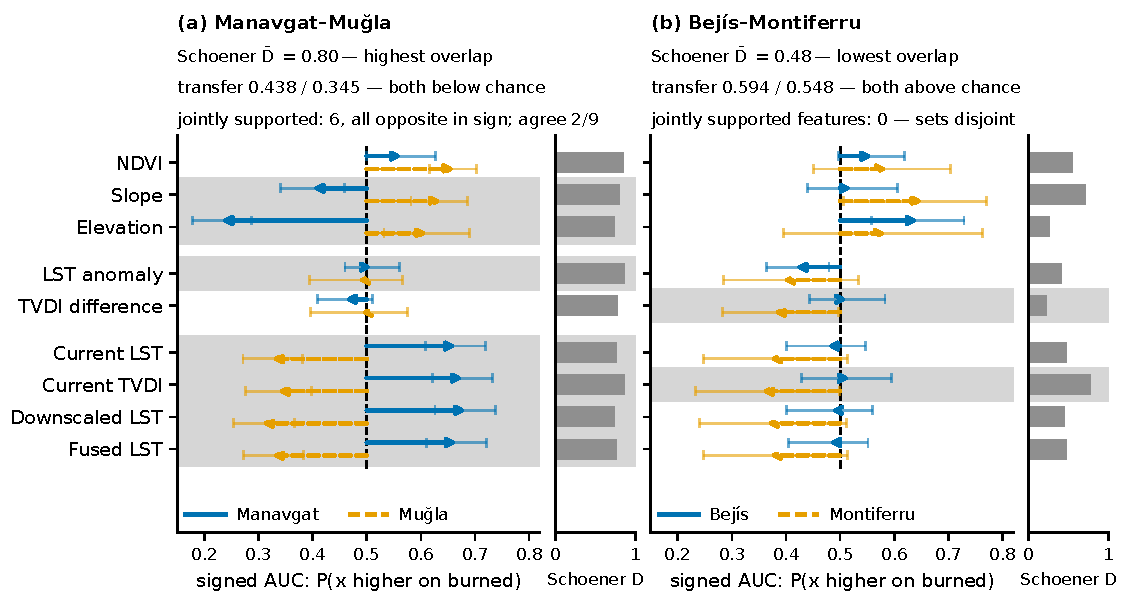
\includegraphics[width=140mm]{figures/fig8_contrast_pairs.pdf}}
  \caption{\textbf{Burned-niche overlap does not determine transfer: the
  contrast pair.} Per-feature signed univariate AUC, the probability that a
  predictor takes a higher value on a burned cell than on an unburned one,
  for the two most informative region pairs, natural-vegetation primary
  population. Arrows run from chance (0.5) to the observed value, so their
  direction is the sign of the association and their length its strength;
  whiskers are 95\% spatial-block ($\approx$5\,km) bootstrap intervals.
  Within each pair the two regions are distinguished by colour, by line style
  (solid for the first region named, dashed for the second) and by vertical
  offset; line style is included because the two hues differ by only 2.30:1 in
  relative luminance and would nearly merge in greyscale.
  \textbf{A filled arrowhead means that region's 95\% interval excludes 0.5, so
  the direction is statistically supported; an open arrowhead means the
  interval contains 0.5 and the direction is not supported.} Rows shaded grey
  are features whose sign disagrees between the two regions. Grey side bars are
  the per-feature Schoener's $D$ overlap.
  \textbf{(a)} Manavgat--Mu\u{g}la, the pair with the \emph{highest} burned-niche
  overlap ($\bar{D}=0.83$), transfers below chance in both directions
  on the frames as drawn (0.470 and 0.401); under the equalised frame of
  Section~\ref{M-sec:4.4} it is 0.551 and 0.510, above chance but still among the
  weakest in the matrix. \textbf{(b)} Bej\'is--Montiferru, the pair with the
  \emph{lowest} overlap ($\bar{D}=0.48$), transfers above chance in both
  directions (0.594 as drawn, 0.669 equalised, and 0.548 against 0.624). High
  niche overlap is therefore not sufficient for transfer, which is an ordinal
  claim on either frame. The arrowhead fill also exposes the coverage limit of the
  supported-agreement index, which is defined only on features whose direction
  is supported in \emph{both} regions: there are two such features in (a)
  (NDVI and elevation) and \textbf{none in (b)}, where the two regions'
  supported sets are disjoint and Montiferru's intervals are wide. Pair (b)
  therefore drops out of the supported-index sample entirely. The index is
  undefined exactly on the pair that most challenges the overlap explanation,
  which is a limitation of the index and not evidence for it.}
  \label{fig:contrast-pairs}
\end{figure}
\end{verbatim}

\section{S5 Target-label recovery curve: what a small labelled budget buys}

\subsection{S5.1 Purpose and status}

The main text establishes that label-free alignment does not close the residual transfer gap, and that the part of that gap not attributable to contiguous spatial holdout is conditional. CORAL and per-region standardisation recover a minority of the gap at best, and degrade most of the directions that transfer above chance without them (\S{}4.5, Section S1.14, \S{}5.5). Within the six directions covered here, the direction that transfers above chance raw is Bejís to Muğla, and it is the direction that both interventions help least. The natural constructive question is therefore what a \emph{small number of target labels} buys, since that is the resource label-free machinery cannot substitute for.

The headline of this analysis is in the main text at Section S1.19. Its ceilings and denominators are computed on the frames as drawn, which \S{}4.4 shows are not comparable across regions; the recovery fractions should be read as within-frame quantities. The full design, the per-budget table and the limits are here, for two reasons. It covers three of the five regions, so it cannot carry a claim at the paper's stated scope; and it requires labelled target cells, so it is not an alternative transfer protocol but a quantification of the price of the failure the main text documents. It is a supplementary sensitivity result, not a proposed method.

\subsection{S5.2 Design}

\textbf{Regions and directions.} Three experiments are used in all six ordered directions: Manavgat 2021, Bejís 2022 and Muğla 2021. Evia is excluded by the frozen configuration on two recorded grounds (\texttt{evia\_\allowbreak{}2021}: out of scope for this analysis; \texttt{evia\_\allowbreak{}2021\_\allowbreak{}extended}: a high-prevalence, different-regime sensitivity control rather than an equal-prevalence primary transfer AOI), and Montiferru does not appear in it. Population, feature sets, forbidden-column set and classifier are the manuscript's primary choices throughout: natural vegetation (\texttt{burnable\_\allowbreak{}tree\_\allowbreak{}shrub\_\allowbreak{}grass} $\wedge$ \texttt{valid\_\allowbreak{}for\_\allowbreak{}modeling}), the ten-feature thermal set as the primary family with the four-feature baseline set as secondary, and the canonical random forest (300 trees, \texttt{min\_\allowbreak{}samples\_\allowbreak{}leaf = 3}, \texttt{class\_\allowbreak{}weight = "balanced"}, \texttt{random\_\allowbreak{}state = 42}).

\textbf{Labelled budget.} The unit of labelling effort is a 10-cell ($\approx$ 5 km) spatial block, assigned before population filtering, identical to the large-block machinery of \S{}3.7. The configuration records why the canonical 2-cell block is not used here: at $\approx$ 1 km a block holds a median of about four cells, which is neither a plausible unit of survey effort nor separable from the evaluation blocks adjacent to it. Budgets are 0, 1, 2, 4, 8, 16 and 32 blocks. Budget 0 is the raw transfer endpoint, which is the source-only model with no target labels. The ceiling is the target-only model evaluated under the same folds.

\textbf{Selection and evaluation.} Blocks are drawn under a fixed tier order (blocks containing both classes, then burned-only, then unburned-only), shuffled within tier by a seed derived as \texttt{blake2b(schema|source|target|outer\_\allowbreak{}fold|repeat)}. The seed is independent of the budget, of the model family and of any result, so no branch of the selection can react to an outcome. Budgets are nested: the 32-block set contains the 16-block set. Evaluation is 5-fold \texttt{StratifiedGroupKFold} grouped on the target's large blocks, in strict mode. Each budget is repeated 10 times with different block draws (the raw and ceiling endpoints once each, being deterministic), for 3,642 unique fits, matching the configuration's own expected count.

\textbf{Uncertainty.} The interval reported is a \textbf{selection interval}: the 2.5th and 97.5th percentiles across the 10 block-selection repeats. It expresses sensitivity to \emph{which} blocks were labelled and nothing else. It is not a bootstrap, it is not a confidence interval, and no \emph{p}-values are produced; the diagnostic enforces this distinction with a forbidden-terminology check. There is consequently no comparable interval on the raw endpoint, which is a single deterministic fit.

\textbf{Recovery fraction.} Defined as (few-shot $-$ raw) / (ceiling $-$ raw), neither clipped nor absolute-valued, so a budget that leaves the model worse than raw transfer reports a negative fraction rather than zero.

\subsection{S5.3 Result}

\begin{table}[htbp]
  \centering
  \footnotesize
  \caption{Few-shot recovery of target ROC-AUC, thermal model, natural-vegetation population. Raw = source-only transfer (budget 0); ceiling = target-only model at the same 10-cell blocking. Values are the mean over 10 block-selection repeats. Read from \texttt{recovery\_\allowbreak{}curve.\allowbreak{}csv}.}
  \label{tab:S22}
  \resizebox{\ifdim\width>\linewidth\linewidth\else\width\fi}{!}{%
  \begin{tabular}{llllllllll}
    \hline
    Direction & Raw & 1 blk & 2 blk & 4 blk & 8 blk & 16 blk & 32 blk & Ceiling & Recovered at 32 \\
    \hline
    Manavgat $\rightarrow$ Bejís & 0.326 & 0.475 & 0.500 & 0.607 & 0.659 & 0.724 & 0.772 & 0.824 & 89 \% \\
    Muğla $\rightarrow$ Bejís & 0.583 & 0.578 & 0.603 & 0.625 & 0.666 & 0.743 & 0.789 & 0.824 & 85 \% \\
    Bejís $\rightarrow$ Manavgat & 0.444 & 0.454 & 0.435 & 0.504 & 0.575 & 0.637 & 0.743 & 0.797 & 85 \% \\
    Muğla $\rightarrow$ Manavgat & 0.401 & 0.413 & 0.420 & 0.447 & 0.471 & 0.517 & 0.626 & 0.797 & 57 \% \\
    Manavgat $\rightarrow$ Muğla & 0.470 & 0.483 & 0.495 & 0.510 & 0.539 & 0.589 & 0.627 & 0.777 & 51 \% \\
    Bejís $\rightarrow$ Muğla & 0.618 & 0.576 & 0.577 & 0.578 & 0.598 & 0.637 & 0.666 & 0.777 & 30 \% \\
    \hline
  \end{tabular}}
\end{table}

Selection intervals are wide at the smallest budgets and narrow at the largest. For Bejís $\rightarrow$ Manavgat they run [0.392, 0.484] at one block against [0.733, 0.748] at 32. See the caution in S5.4 on why the upper-budget intervals are narrow.

Three observations follow, and only the first is comfortable.

\textbf{The largest budget tested recovers most of the gap in three of six directions.} Thirty-two blocks carry on average 2,700 to 3,000 labelled cells, roughly 7 to 20 \% of the target's natural-vegetation population depending on the region. At that budget three directions stand at 85 to 89 \% of their target-only ceiling: Manavgat $\rightarrow$ Bejís and Bejís $\rightarrow$ Manavgat started below chance, Muğla $\rightarrow$ Bejís at 0.583, above it. The residual the main text documents is therefore expensive but not structural: it is a shortage of target-conditional information, and target labels supply exactly that. That budget should not be described as modest. Limit 4 below gives the reason: for these AOIs the top budget already contains most of the target's burned cells.

\textbf{The recovery is slow where the transfer is worst.} The two directions into Muğla and Manavgat from Muğla reach only 51 to 57 \% at the top budget. These are the directions whose raw transfer sits furthest below the ceiling, and Muğla $\rightarrow$ Manavgat is still below 0.5 AUC after 8 labelled blocks. A larger concept gap costs more labels, not the same labels.

\textbf{Small budgets actively hurt the one direction that already transfers.} Bejís $\rightarrow$ Muğla is the pair that transfers above chance raw (0.618), and it is the pair few-shot recalibration helps least: the curve is \emph{negative} at 1, 2, 4 and 8 blocks ($-$0.043 to $-$0.021 AUC), only overtakes raw at 16, and reaches 30 \% at 32, the worst of the six. This is the same asymmetry the main text reports for label-free adaptation (\S{}4.5): where the source model already carries a usable conditional relationship, a small target sample perturbs it before it can replace it. The mechanism differs, since here the target labels are real information rather than a covariate rescaling. The direction of the effect is nevertheless the same, and it is the one direction where the intervention is a liability at every budget a field campaign would plausibly afford.

\subsection{S5.4 Methodological limits}

These are stated so the analysis is not read as more than it is.

\begin{enumerate}
  \item \textbf{Three regions, six directions.} Evia and Montiferru are absent, so this covers six of the twenty directed pairs in the main analysis and cannot speak to the five-region scope.
  \item \textbf{It requires labelled target cells.} The budget axis is labels in the target region. Nothing here is a label-free method and nothing here weakens the paper's negative result about label-free alignment. It prices that result.
  \item \textbf{No joint analysis with the conditional index.} Whether the labelled budget needed to reach a given recovery fraction is predicted by the conditional sign-agreement index of \S{}3.11 was not computed. With six directions it would in any case be a description rather than a test.
  \item \textbf{The interval is a selection interval, and it narrows for a reason that is not precision.} Bejís holds only 15 blocks containing both classes and 19 containing any burned cell; Manavgat 26 and 28; Muğla 60 and 70. At 16 and 32 blocks the tiered draw has nearly exhausted the both-class blocks, so repeats select almost the same set. The mean labelled-positive count into Bejís is identically 860.0 at 16 blocks and 880.0 at 32 across both source regions. The narrow upper-budget intervals therefore reflect a saturated selection pool, not a well-estimated quantity, and the top budget is not a small budget for these AOIs: 880 of Bejís's 1,100 burned cells are inside it.
  \item \textbf{The ceiling is the 10-cell-block target-only value}, not the $\approx$ 1 km within-region headline reported in the main paper, and is correspondingly lower (0.777 to 0.824 against 0.859 to 0.918). Recovery fractions are only interpretable against this matched-blocking ceiling.
  \item \textbf{Ceiling reproduction verified for all three targets.} Manavgat, Bejís and Muğla all reproduce the frozen large-block artefacts exactly, at an absolute difference of 0.0 against a 10$^{-9}$ tolerance in both families. An earlier draft of this supplement recorded Muğla as unverified, because at that time no frozen block-10 artefact had been located for it; one is now referenced in the export and the corresponding validator check passes.
  \item \textbf{Provenance.} The export of record was regenerated on 2026-08-14 at commit \texttt{6d7a6a71} under scikit-learn 1.9.0, pandas 3.0.2 and NumPy 2.4.4 --- the same scikit-learn version to which every other number in this paper is fixed. Its validator reports \textbf{67 PASS, 0 FAIL and 0 SKIPPED}. Two files in the export directory, \texttt{repeat\_\allowbreak{}metrics.\allowbreak{}csv} and \texttt{oof\_\allowbreak{}predictions.\allowbreak{}parquet}, retain their 2026-08-03 timestamps and were not regenerated; every value quoted in Table~\ref{tab:S1} was checked against the regenerated export.
\end{enumerate}

\subsection{S5.5 Figure}

A recovery curve is the natural presentation, and it is prepared from \texttt{recovery\_\allowbreak{}curve.\allowbreak{}csv} (thermal family, \texttt{metric = roc\_\allowbreak{}auc}). Budget goes on a log-2 axis and target ROC-AUC on the ordinate. Each direction is one line, the selection interval is drawn as a band, and each direction's ceiling is a horizontal reference. Numbers are as in Table~\ref{tab:S1}.
\bibliographystyle{elsarticle-harv}
\bibliography{../REFERENCES}
\end{document}
